%!TEX root = ..\Thesis.tex

\glsresetall

\chapter{Statistical Analysis}\label{chap:StatisticalAnalysis}
\begin{quote}
\emph{The results of this chapter ...}\vfill{}
\end{quote}



\section{Introduction  - Statistical analysis}


Errors-in-variables (EIV) are linear estimation problems in which the regression matrix and the regressor are perturbed \cite{VanHuffel91Book}, \cite{Markovsky07overview}.
In structured EIV problems, the regression matrix has a given structure that depends on the problem formulation.
Hankel, Toeplitz, or other application-specific matrices appear in problems of metrology \cite{Markovsky15cep}, system identification \cite{Soderstrom07}, image restoration \cite{Feiz17}, nuclear magnetic resonance spectroscopy \cite{Cai16}, direction-of-arrival estimation \cite{Pan18}, and time-of-arrival estimation \cite{Jia18}.

In metrology, the direct estimation of the input from the sensor transient response is formulated as a structured EIV problem.
The only observed signal is the sensor output.
To estimate a step input, the regression matrix, and the regressor are built from the step response observations \cite{Markovsky15cep}, and
the structure in the regression matrix is block-Hankel.
This data-driven estimation methodology reduces the estimation time of the classical two-stage approach where a sensor model is first identified, and later the input is estimated using the sensor model \cite{Azam15, Niedzwiecki16a}.
%The problem is EIV because the perturbation of the sensor response gets into the regression matrix.

Total least-squares (TLS) is the typical estimator for unstructured EIV problems and is consistent when the perturbations have zero mean, and the covariance is a given positive definite matrix.
When the perturbations are i.i.d. normally distributed, the solution of the TLS is equivalent to that of the maximum likelihood estimator (ML) \cite{Markovsky07overview}. 
For structured EIV problems, the TLS estimator does not give general results since each specific structure requires a particular treatment \cite{VanHuffel07TLSeditorial}, and the ML estimator leads to non-convex optimization problems where finding the global optimum is not guaranteed \cite{Rhode14recursive}.
Moreover, the computational complexity of TLS and ML inhibits real-time implementation to solve structured EIV problems. 

The least-squares (LS) estimator is a suboptimal but simple solution to structured EIV problems that admits a recursive form for easy real-time implementations.
Some of the reported works that propose LS estimators for structured EIV problems include 
the design of a fast algorithm for matrices with small displacement rank \cite{Mastronardi07fast},
the study of the estimator consistency \cite{Palanthandalam10parameter},
the determination of the bias, and the mean squared error of the parameter estimates in the identification of AR models \cite{Kiviet12high} \cite{Kiviet14improved}, and
a discussion of the causes of bias and inconsistency in homogeneous estimators \cite{Yeredor04homogeneous}.

 In measurement applications, it is highly relevant to assess the uncertainty of the input estimate.
The uncertainty of the reported LS estimators for structured EIV problems has not been addressed, and then, remains unknown.
The estimator uncertainty is expressed using the estimation bias and covariance \cite{Pintelon12Book}.
To know the LS estimator uncertainty, we quantified the bias and the covariance of the LS solution of EIV problems in the unstructured and structured cases. 
This extends the perturbation analysis of the LS estimator of unstructured and uncorrelated problems that was investigated in \cite{Stewart90SPT} and in \cite{Vaccaro94}.
This paper presents a study of the statistics of the LS estimate of unstructured and structured EIV problems. 
 We provide a discussion of the unstructured case as a reference, to get an insight of the impact that the structure of the regression matrix and the correlation between the regression matrix and the regressor perturbations have on the uncertainty of the LS estimate.
The structured case is motivated by the metrology estimation problem \cite{Markovsky15cep}, where the EIV problem has a Hankel structure, and the perturbations are correlated.
The study of the metrology input estimate illustrates a methodology to conduct statistical analysis for any structured EIV problem.
The mathematical expectation of the second-order Taylor series expansion of the LS estimate boils down to expressions that quantify the first and second-order moments of the LS estimate.
Via Monte Carlo simulations, we validated the accuracy of the bias, and the covariance approximations.
The derived approximations predict the LS estimate bias, and the covariance, for given sample size and perturbation level.
The predicted variance gives the uncertainty of the LS estimate.
We observed that, for the step input estimation problem, the mean squared error of the LS estimate is near to the minimum variance limit given by the Cram\'er-Rao lower bound of the structured EIV problem.
 By following this methodology, the bias and variance of the solutions of EIV problems with other structures is determined, and therefore, the uncertainty of the estimate.




\section{Statistical analysis}


For an overdetermined system of linear equations, the least-squares (LS) solution is given by
\begin{equation} \widehat{\mathbf{x}} = \widetilde{\mathbf{K}}^\dagger \widetilde{\mathbf{y}} = ( \widetilde{\mathbf{K}}^\top \widetilde{\mathbf{K}} )^{-1} \widetilde{\mathbf{K}}^\top \widetilde{\mathbf{y}} , \label{eqn:xhat} \end{equation}
where $\widetilde{\mathbf{K}}^\dagger$ is the pseudo-inverse of $\widetilde{\mathbf{K}}$.
The objective of the statistical analysis is to obtain the bias and the covariance of the solution $\widehat{\mathbf{x}}$.
The bias and the covariance are computed using the mathematical expectation operator $\mathbb{E}\{\cdot\}$.
First we substitute (\ref{eqn:y0plusnoise}) and (\ref{eqn:K0plusnoise}) in (\ref{eqn:xhat}) obtaining
\begin{equation*} \widehat{\mathbf{x}} = \left( (\mathbf{K}+\mathbf{E})^\top (\mathbf{K}+\mathbf{E})  \right)^{-1} (\mathbf{K}+\mathbf{E})^\top (\mathbf{y}+\bm{\epsilon}), \end{equation*} 
which is equivalent to
\begin{equation} \widehat{\mathbf{x}} = \left( \mathbf{I} + \mathbf{M} \right)^{-1} \mathbf{Q}^{-1} (\mathbf{K}+\mathbf{E})^\top (\mathbf{y}+\bm{\epsilon}), \label{eqn:1steq} \end{equation} 
where 
\begin{equation} \mathbf{Q} = \mathbf{K}^\top \mathbf{K}, \quad \text{and} \quad \mathbf{M} = \mathbf{Q}^{-1} ( \mathbf{K}^\top \mathbf{E} + \mathbf{E}^\top \mathbf{K} + \mathbf{E}^\top \mathbf{E} ). \end{equation} 
Applying a second-order Taylor expansion of the inverse matrix
\begin{equation} (\mathbf{I} + \mathbf{M})^{-1} \approx \mathbf{I} - \mathbf{M} + \mathbf{M}^2, \label{eqn:TseriesExp} \end{equation} 
that is valid when the SNR is sufficiently high, and therefore $\mathbf{E}$ and $\mathbf{M}$ are small, satisfying the constraint on the spectral radius $\| \mathbf{M} \| < 1$. 
The neglected term in the Taylor series expansion is of the order $O(\Vert M \Vert^3)$.
We can express the estimate as
\begin{equation} \widehat{\mathbf{x}} \approx \left( \mathbf{I} - \mathbf{M} + \mathbf{M}^2 \right) \mathbf{Q}^{-1} (\mathbf{K}+\mathbf{E})^\top (\mathbf{y}+\bm{\epsilon}). \label{eqn:xhatexp} \end{equation} 

Now that the perturbation variables $\bm{\epsilon}$ and $\mathbf{E}$ are no longer inside an inverse matrix, we can compute the mathematical expectation of expressions derived from the Taylor series approximation (\ref{eqn:xhatexp}) of $\widehat{\mathbf{x}}$. 
The bias of the estimate $\widehat{\mathbf{x}}$ is obtained from
\begin{equation} \mathbf{b} \left(\widehat{\mathbf{x}} \right) = \bm{\mu}\left(\widehat{\mathbf{x}} \right) - \mathbf{x}, \label{eqn:biasdef} \end{equation}
where $\bm{\mu} \left(\widehat{\mathbf{x}} \right) = \mathbb{E} \left\{ \widehat{\mathbf{x}} \right\}$, and $\mathbf{x} = \mathbf{K}^\dagger \mathbf{y} = \mathbf{Q}^{-1} \mathbf{K}^\top \mathbf{y}$ is the true value.
The covariance of the estimate $\widehat{\mathbf{x}}$ is obtained from
\begin{equation} \begin{aligned} \mathbf{C} \left( \widehat{\mathbf{x}} \right) & = \mathbb{E} \left\{ \left( \widehat{\mathbf{x}} - \bm{\mu} \right) \left( \widehat{\mathbf{x}} - \bm{\mu} \right)^\top \right\} . \end{aligned} \label{eqn:covdef} \end{equation} 

The terms derived from (\ref{eqn:xhatexp}) that do not contribute to the bias and to the covariance are filtered out by the mathematical expectation operator considering the following general rules that are valid regardless of the existence of structure in the regression problem: 
\begin{itemize}
	\item the expected values $\mathbb{E} \{ \mathbf{E} \} = \mathbf{0}$, and $\mathbb{E} \{ \bm{\epsilon} \} = \mathbf{0}$, since $\mathbf{E}$ and $\bm{\epsilon}$ are zero-mean random variables, and
	\item the expected values of odd order moments, such as $\mathbb{E} \{ \mathbf{E}^\top \mathbf{E} \mathbf{E}^\top \}$, are zero.
\end{itemize}
Moreover, the second-order approximation disregards moments of order four and higher.

After removing the terms with negligible expected value, we have expressions that are approximations of the LS estimation bias and covariance. 
These expressions are different depending on the type of EIV problem considered.
Subsections 3.1 and 3.2 describe the resulting expressions for the unstructured and structured EIV problems, respectively.
The perturbations in the considered unstructured EIV problem are independent.
Comparing the expressions that result from the statistical analysis, we get an insight of what is the impact that the structure and the correlation have on the LS solution of the structured EIV problem.

\subsection{Bias and covariance of the LS estimator for an unstructured EIV problem with uncorrelated noise}
% We consider the unstructured matrix $\mathbf{K} \in \mathbb{R}^{\left(T-n\right) \times \left(n+1\right)}$ with the same dimensions as the structured EIV case.

First, the statistics of the least squares estimator (\ref{eqn:xhat}) of an unstructured EIV problem is discussed, 
provided that the perturbations of the regression matrix and the regressor are i.i.d. normally distributed with zero mean, and variances $\sigma_{\mathbf{E}}^2$ and $\sigma_{\bm{\epsilon}}^2$, respectively.
Therefore, the terms in the Taylor series expansion (\ref{eqn:xhatexp}) that contain products of $\mathbf{E}$ and $\bm{\epsilon}$ have zero expected value.
 After removing the terms without contribution to the bias, and to the covariance, with the mathematical expectation operator,
the analytic approximation of the bias (\ref{eqn:biasdef}) is given by 
\begin{equation} \begin{aligned} \mathbf{b}_{\mathrm{p}} \left( \widehat{\mathbf{x}} \right) & \approx \sigma_{\mathbf{E}}^2 \left( 2 + 2n - T \right) \mathbf{Q}^{-1} \mathbf{x} , \end{aligned} \label{eqn:biasEu} \end{equation}
and the covariance (\ref{eqn:covdef}) is approximated by 
\begin{equation} \begin{aligned} \mathbf{C}_{\mathrm{p}} \left( \widehat{\mathbf{x}} \right) & \approx \sigma_{\bm{\epsilon}}^2 \ \mathbf{Q}^{-1} + \sigma_{\mathbf{E}}^2 \ \mathrm{trace} \left( \mathbf{x} \mathbf{x}^\top \right) \mathbf{Q}^{-1} - \sigma_{\mathbf{E}}^4 \left( 2 + 2n - T \right)^2 \ \mathbf{Q}^{-1} \mathbf{x} \mathbf{x}^\top \mathbf{Q}^{-1} , \end{aligned} \label{eqn:varEu} \end{equation}
where the subscript $\mathrm{p}$ stands for prediction of the bias and covariance.
The derivation of equations (\ref{eqn:biasEu}) and (\ref{eqn:varEu}) is described in Appendix 1.
We use the results described in \cite{Vaccaro94} \S 3 and \cite{Stewart90SPT} \S 2.1 for the expected values of products of unstructured matrices with perturbations.
Equations (\ref{eqn:biasEu}) and (\ref{eqn:varEu}) depend on the unobservable true values $\mathbf{x}$, $\mathbf{K}$, and on the variance of the perturbations.
The observed variables are $\widetilde{\mathbf{y}}$, $\widetilde{\mathbf{K}}$, and from them we compute $\widehat{\mathbf{x}}$.
It is proposed to directly substitute the observed variables in the analytic expressions.
The substitution gives an approximation of the estimate bias and covariance using the observed data.
We have then
\begin{equation} \begin{aligned} \widetilde{\mathbf{b}}_{\mathrm{p}} \left( \widehat{\mathbf{x}} \right) & \approx \sigma_{\mathbf{E}}^2 \left( 2 + 2n - T \right) \widetilde{\mathbf{Q}}^{-1} \widehat{\mathbf{x}} , \end{aligned} \label{eqn:biasEuST} \end{equation}
\begin{equation} \begin{aligned} \widetilde{\mathbf{C}}_{\mathrm{p}} \left( \widehat{\mathbf{x}} \right) & \approx \sigma_\epsilon^2 \ \widetilde{\mathbf{Q}}^{-1} + \sigma_{\mathbf{E}}^2 \ \mathrm{trace} \left( \widehat{\mathbf{x}} \widehat{\mathbf{x}}^\top \right) \widetilde{\mathbf{Q}}^{-1} - \sigma_{\mathbf{E}}^4 \left( 2 + 2n - T \right)^2 \widetilde{\mathbf{Q}}^{-1} \widehat{\mathbf{x}} \widehat{\mathbf{x}}^\top \widetilde{\mathbf{Q}}^{-1} . \end{aligned} \label{eqn:varEuST} \end{equation}
In order to have a prediction of the estimate bias and covariance, the variances $\sigma_{\mathbf{E}}^2$ and $\sigma_{\bm{\epsilon}}^2$ and the observed variables $\widetilde{\mathbf{y}}$, $\widetilde{\mathbf{K}}$, and $\widehat{\mathbf{x}}$ are needed.


\subsection{Bias and covariance of the LS estimator for a structured EIV problem with noise correlation}

This subsection describes the statistics of a structured EIV problem with correlation between the perturbations of the regression matrix and the regressor. 
The structured EIV problem is given by the step input estimation method (\ref{eqn:min_ls}).
The correlation is a consequence of the construction of the block-Hankel matrix in the regression matrix $\widetilde{\mathbf{K}}$ with the first difference of the elements in the regressor $\widetilde{\mathbf{y}}$.

The mathematical expectation operator is applied to the Taylor series expansion of the LS estimate (\ref{eqn:xhatexp}).
After removing the terms with negligible expected value, and considering the structure of matrix $\mathbf{K}$, the estimation bias (\ref{eqn:biasdef}) is approximated by 
\begin{equation} \begin{aligned} \mathbf{b}_{\mathrm{p}} \left( \widehat{\mathbf{x}} \right) & \approx \mathbf{Q}^{-1} \left( \left( \mathbf{K}^\top \mathbf{B}_1 - \mathbf{B}_2 \right) x - \left( \mathbf{K}^\top \mathbf{B}_3 - \mathbf{B}_4 \right) \right) , \end{aligned} \label{eqn:biasE} \end{equation}
whereas, the estimation covariance (\ref{eqn:covdef}) is approximated by 
\begin{equation} \begin{aligned} \mathbf{C}_{\mathrm{p}} \left( \widehat{\mathbf{x}} \right) & \approx \mathbf{K}^\dagger \left( \sigma_{\bm{\epsilon}}^2 \mathbf{I}_{T-n} + \mathbf{C}_1 - \mathbf{C}_2 - \mathbf{C}_2^\top \right) \mathbf{K}^{\dagger \top} - \mathbf{b}_{\mathrm{p}} \left( \widehat{\mathbf{x}} \right) \mathbf{b}_{\mathrm{p}}^\top \left( \widehat{\mathbf{x}} \right) , \end{aligned} \label{eqn:varE} \end{equation}
where $\mathbf{B}_1 = \mathbb{E} \Big\{ \mathbf{E} \mathbf{K}^\dagger \mathbf{E} \Big\}$, $\mathbf{B}_2 = \mathbb{E} \Big\{ \mathbf{E}^\top \mathbf{P}_\perp \mathbf{E} \Big\}$, $\mathbf{B}_3 = \mathbb{E} \Big\{ \mathbf{E} \mathbf{K}^\dagger \bm{\epsilon} \Big\}$, $\mathbf{B}_4 = \mathbb{E} \Big\{ \mathbf{E}^\top \mathbf{P}_\perp \bm{\epsilon} \Big\}$, $\mathbf{C}_1 = \mathbb{E} \Big\{ \mathbf{E} \mathbf{x} \mathbf{x}^\top \mathbf{E}^\top \Big\}$, $\mathbf{C}_2 = \mathbb{E} \Big\{ \mathbf{E} \mathbf{x} \bm{\epsilon}^\top \Big\}$, $\mathbf{P} = \mathbf{K} \mathbf{K}^\dagger$, and $\mathbf{P}_\perp = \mathbf{I} - \mathbf{P}$. 
The derivation of equations (\ref{eqn:biasE}) and (\ref{eqn:varE}) is described in Appendix 1.
The expected values $\mathbf{B}_1$, $\mathbf{B}_2$, $\mathbf{B}_3$, $\mathbf{B}_4$, $\mathbf{C}_1$ and $\mathbf{C}_2$ are obtained using the results of Lemma \ref{lem:lemma1}.

\newtheorem{thm}{Theorem}
\newtheorem{lem}[thm]{Lemma}
\newproof{pf}{Proof}

\small
% <how to set font size here to 10 px ? />

\begin{lem}{\small}\label{lem:lemma1}
Let $\mathbf{E} \in {\rm I\!R}^{\left(T-n\right) \times \left(n+1\right)}$ be the partitioned matrix 
\[ \mathbf{E} = \begin{bmatrix} \mathbf{0}_{T-n \times 1} & \bm{\mathcal{H}}(\bm{\epsilon}) \mathbf{D}_{n+1 \times n}^{1,0} \end{bmatrix}, \]
 where $\bm{\mathcal{H}}(\bm{\epsilon}) \in {\rm I\!R}^{\left(T-n\right) \times \left(n+1\right)}$ is the block-Hankel matrix of $T-n$ rows and $n$ columns
\[ \bm{\mathcal{H}}(\bm{\epsilon}) = \begin{bmatrix} \epsilon(0) & \epsilon(1) & \cdots & \epsilon(n) \\ \epsilon(1) & \epsilon(2) & \cdots & \epsilon(n+1) \\ \vdots & \vdots & & \vdots \\ \epsilon(T-n-1) & \epsilon(T-n) & \cdots & \epsilon(T-1) \end{bmatrix} , \]
constructed from samples of the i.i.d. normally distributed random variable $\bm{\epsilon} \sim \mathcal{N}(0, \sigma_{\bm{\epsilon}}^2)$.
Let $\mathbf{D}_{r \times c}^{1,k}$ and $\mathbf{D}_{r \times c}^{2,k}$ be the first and second-order finite differences matricial operators of dimensions $r \times c$ starting from the subdiagonal $k$, for example, 
\[ \mathbf{D}_{4 \times 3}^{1,-1} = \begin{bmatrix} 0 & 0 & 0 \\ -1 & 0 & 0 \\ 1 & -1 & 0 \\ 0 & 1 & -1 \end{bmatrix}, \ \mathbf{D}_{4 \times 3}^{2,0} = \begin{bmatrix}-1 & 0 & 0 \\ 2 & -1 & 0 \\ - 1 & 2 & -1 \\ 0 & -1 & 2 \end{bmatrix} . \]
For a compatible deterministic matrix $\mathbf{A}$, or vector $\mathbf{a}$, the following expected values hold.
\begin{equation*} \begin{aligned} 
& \mathbb{E} \left\{ \mathbf{E} \mathbf{A} \mathbf{E} \right\} = \mathbf{Z}, \
\text{where} \ \mathbf{z}_{i1} = \mathbf{0}, \ \text{and} \ 
z_{ij} = \sigma_{\bm{\epsilon}}^2 \ \mathrm{Tr} \left( \mathbf{A} \begin{bmatrix} \mathbf{0}_{T-n} & \mathbf{D}_{T-n \times n}^{2, j-i} \end{bmatrix} \right), \
\text{for} \ i = 1, \cdots, T-n, \ \text{and} \ j = 2, \cdots, n+1. \\
& \mathbb{E} \left\{ \mathbf{E}^\top \mathbf{A} \mathbf{E} \right\} = \mathbf{Z}, \ 
\text{where} \ \mathbf{z}_{1j} = \mathbf{0}, \ \mathbf{z}_{i1} = \mathbf{0}, \ \text{and} \ 
z_{ij} = \sigma_{\bm{\epsilon}}^2 \ \mathrm{Tr} \left( \mathbf{A} \ \mathbf{D}_{T-n \times T-n}^{2, j-i+1} \right) , \
\text{for} \ i = 2, \cdots, n+1, \ \text{and} \ j=2, \cdots, n+1 . \\ 
& \mathbb{E} \left\{ \mathbf{E} \mathbf{A} \mathbf{E}^\top \right\} = \mathbf{Z}, \
\text{where} \ z_{ij} = \sigma_{\bm{\epsilon}}^2 \ \mathrm{Tr} \left( \mathbf{A} \begin{bmatrix} 0 & \mathbf{0}_{n}^\top \\ \mathbf{0}_{n} & \mathbf{D}_{n \times n}^{2, j-i+1} \end{bmatrix} \right), \
\text{for} \ i = 1,\cdots,T-n, \ \text{and} \ j=1,\cdots,T-n. \\ 
& \mathbb{E} \left\{ \mathbf{E} \mathbf{A} \bm{\epsilon} \right\} = \mathbf{z}, \
\text{where} \ z_i = \sigma_{\bm{\epsilon}}^2 \ \mathrm{Tr} \left( \mathbf{A} \begin{bmatrix} \mathbf{0}_{T-n} & \mathbf{D}_{T-n \times n}^{1,n+1-i} \end{bmatrix} \right) , \
\text{for} \ i = 1,\cdots,T-n . \\
& \mathbb{E} \left\{ \mathbf{E}^\top \mathbf{A} \bm{\epsilon} \right\} = \mathbf{z}, \
\text{where} \ z_1 = 0, \ \text{and} \ z_i = \sigma_{\bm{\epsilon}}^2 \ \mathrm{Tr} \left( \mathbf{A} \ \mathbf{D}_{T-n \times T-n}^{1, n+2-i} \right), \
\text{for} \ i = 2,\cdots,n+1 . \\
& \mathbb{E} \left\{ \mathbf{E} \mathbf{a} \bm{\epsilon}^\top \right\} = \mathbf{Z}, \
\text{where each column} \ \mathbf{Z}_{j} = - \sigma_{\bm{\epsilon}}^2 \ \mathbf{D}_{T-n \times n+1}^{1,-j} \mathbf{R}_{n+1} \ \mathbf{a} , \
\text{for} \ j = 1,\cdots,T-n , \ \text{with} \ \mathbf{R}_{n+1} = \begin{bmatrix} & \mathbf{R}_n \\ 0 \end{bmatrix} , \\ & \quad
\text{where} \ \mathbf{R}_n \ \text{is a reversal matrix.}
\end{aligned} \end{equation*} 
\end{lem}

\normalsize

The proof of the lemma is given in Appendix 2.

The matrices $\mathbf{B}_1$, $\mathbf{B}_2$, $\mathbf{B}_3$, $\mathbf{B}_4$, $\mathbf{C}_1$ and $\mathbf{C}_2$ are considered in the different cases of Lemma \ref{lem:lemma1}.
Each expected value in the lemma is a matrix, or a vector, whose elements are found following the indicated operations.
These operations mainly compute the trace of a product of the corresponding deterministic matrix $\mathbf{A}$, and a matrix constructed from the finite differences matricial operator, which can be of first order $\mathbf{D}^{1}$ or of second order $\mathbf{D}^{2}$.
The total number of operations in the computation of the bias and the covariance is $O\left( T^3 + n^2 \right)$, but this order can be reduced since the $\mathbf{D}$ matrices are sparse.

The formulas for the bias and covariance (\ref{eqn:biasE}) and (\ref{eqn:varE}) depend on the perturbation variance and on the unobservable variables $\mathbf{x}$ and $\mathbf{K}$.
The substitution of the observed variables in the expression gives an approximation of the estimate bias and covariance based on the observed system response.
We have then
\begin{equation} \begin{aligned} \mathbf{b}_{\widetilde{\mathrm{p}}} \left( \widehat{\mathbf{x}} \right) & \approx \widetilde{\mathbf{Q}}^{-1} \left( \left( \widetilde{\mathbf{K}}^\top \widetilde{\mathbf{B}}_1 - \widetilde{\mathbf{B}}_2 \right) \widehat{\mathbf{x}} - \left( \widetilde{\mathbf{K}}^\top \widetilde{\mathbf{B}}_3 - \widetilde{\mathbf{B}}_4 \right) \right), \end{aligned} \label{eqn:biasST} \end{equation}
and
\begin{equation} \begin{aligned} \mathbf{C}_{\widetilde{\mathrm{p}}} \left( \widehat{\mathbf{x}} \right) & \approx \widetilde{\mathbf{K}}^\dagger \left( \sigma_{\bm{\epsilon}}^2 \mathbf{I}_{T-n} + \widetilde{\mathbf{C}}_1 - \widetilde{\mathbf{C}}_2 - \widetilde{\mathbf{C}}_2^\top \right) \widetilde{\mathbf{K}}^{\dagger \top} - \mathbf{b}_{\widetilde{\mathrm{p}}} \left( \widehat{\mathbf{x}} \right) \mathbf{b}_{\widetilde{\mathrm{p}}}^\top \left( \widehat{\mathbf{x}} \right) , \end{aligned} \label{eqn:varST} \end{equation}
where $\widetilde{\mathbf{B}}_1 = \mathbb{E} \Big\{ \mathbf{E} \widetilde{\mathbf{K}}^\dagger \mathbf{E} \Big\}$, $\widetilde{\mathbf{B}}_2 = \mathbb{E} \Big\{ \mathbf{E}^\top \widetilde{\mathbf{P}}_\perp \mathbf{E} \Big\}$, $\widetilde{\mathbf{B}}_3 = \mathbb{E} \Big\{ \mathbf{E} \widetilde{\mathbf{K}}^\dagger \bm{\epsilon} \Big\}$, $\widetilde{\mathbf{B}}_4 = \mathbb{E} \Big\{ \mathbf{E}^\top \widetilde{\mathbf{P}}_\perp \bm{\epsilon} \Big\}$, $\widetilde{\mathbf{C}}_1 = \mathbb{E} \Big\{ \mathbf{E} \widehat{\mathbf{x}} \widehat{\mathbf{x}}^\top \mathbf{E}^\top \Big\}$, $\widetilde{\mathbf{C}}_2 = \mathbb{E} \Big\{ \mathbf{E} \widehat{\mathbf{x}} \bm{\epsilon}^\top \Big\}$, $\widetilde{\mathbf{C}} = \widetilde{\mathbf{K}}^\top \widetilde{\mathbf{K}}$, $\widetilde{\mathbf{P}} = \widetilde{\mathbf{K}} \widetilde{\mathbf{K}}^\dagger$, and $\widetilde{\mathbf{P}}_\perp = \mathbf{I} - \widetilde{\mathbf{P}}$.

\subsection{Cram\'er-Rao lower bound of the structured errors-in-variables problem}

The Cram\'er-Rao lower bound (CRLB) provides the lower limit on the variance of the estimate
\begin{equation} \mathrm{CRLB}(\mathbf{x}) = \left( \mathbf{I} + \frac{\partial \mathbf{b} (\widehat{\mathbf{x}}) }{\partial (\widehat{\mathbf{x}})} \right)^\top \mathbf{Fi}^{-1}(\mathbf{x}) \left( \mathbf{I} + \frac{\partial \mathbf{b} (\widehat{\mathbf{x}}) }{\partial (\widehat{\mathbf{x}})} \right), \label{eqn:CRLB} \end{equation}
where $\mathbf{b} (\widehat{\mathbf{x}})$ is the bias of the estimate and $\mathbf{Fi}(\widehat{\mathbf{x}})$ is the Fisher information matrix \cite{Pintelon12Book}.
The Fisher information matrix is defined as the expected value of the Hessian of the negative likelihood function 
\begin{equation} \mathbf{Fi}(x) = - \mathbb{E} \left\{ \frac{\partial ^2 l (\widehat{\mathbf{x}}) }{\partial \widehat{\mathbf{x}}^2 } \right\}, \end{equation}
where the partial derivatives are evaluated in $\widehat{\mathbf{x}} = \mathbf{x}$.

The minimization problem (\ref{eqn:min_ls}) is equivalent to a structured EIV problem that can be expressed as a linear in the measurements problem \cite{Pintelon12Book}
\begin{equation} e (\widehat{\mathbf{x}}, \widetilde{\mathbf{z}}) = \mathbf{M}_1( \widehat{\mathbf{x}} ) \ \widetilde{\mathbf{z}} = \begin{bmatrix} \mathbf{I}_{T-n} & - \widehat{\mathbf{x}}^T \otimes \mathbf{I}_{T-n} \end{bmatrix} \begin{bmatrix} \widetilde{\mathbf{y}} \\ \mathrm{vec} ( \widetilde{\mathbf{K}} ) \end{bmatrix} = 0 . \label{eqn:M1vecyK} \end{equation}
where $\widetilde{\mathbf{z}} = \mathbf{z} + \epsilon_{\mathbf{z}}$.
The CRB requires that the true model $\mathbf{M}_1( \mathbf{x} ) \ \mathbf{z} = 0$ exists.
Under the assumption of the measurement perturbation $\epsilon_{\mathbf{z}}$ being normally distributed with covariance matrix $\mathbf{C}_{\mathbf{z}}$, the loglikelihood function of the structured EIV problem is
\begin{equation} \ln{ l(\widetilde{\mathbf{z}}, \widehat{\mathbf{z}}, \widehat{\mathbf{x}}) } = - \frac{1}{2} \left( \widetilde{\mathbf{z}} - \widehat{\mathbf{z}} \right)^\top \mathbf{C}_{\mathbf{z}}^{-1} \left( \widetilde{\mathbf{z}} - \widehat{\mathbf{z}} \right) + \mathrm{constant}, \end{equation}
where $\widehat{\mathbf{z}}$ are parameters of the measurements $\widetilde{\mathbf{z}}$ that have to be estimated and satisfy $\mathbf{M}_1( \widehat{\mathbf{x}} ) \ \widehat{\mathbf{z}} = 0$.
The size of the Fisher information matrix $\mathbf{Fi}(\mathbf{x}, \mathbf{z})$ depends on the number of unknowns in $\widehat{\mathbf{z}}$ and grows with the sample size.
Moreover, in Chapter 19 of \cite{Pintelon12Book} it is shown that the Fisher information matrix $\mathbf{Fi}(\mathbf{x})$ can be obtained from $\mathbf{Fi}(\mathbf{x}, \mathbf{z})$ after doing inversion by parts, giving
\begin{equation} \mathbf{Fi}(\mathbf{x}) = \left( \frac{\partial e (\widehat{\mathbf{x}}, \mathbf{z}) }{\partial \mathbf{x} } \right)^\top \left( \mathbf{M}_1( \mathbf{x} ) \ \mathbf{C}_{\mathbf{z}} \ \mathbf{M}_1^\top( \mathbf{x} ) \right)^{-1} \left( \frac{\partial e (\widehat{\mathbf{x}}, \mathbf{z}) }{\partial \mathbf{x} } \right) 
 , \label{eqn:FIM} \end{equation} 
where the partial derivatives are evaluated at the true values $\mathbf{x}$, and the covariance matrix of the measurements is
\begin{equation} \mathbf{C}_{\mathbf{z}} = \sigma_{\epsilon}^2 \begin{bmatrix} \mathbf{I}_{T-n} & \mathbf{0}_{T-n} & \mathbf{D}_{T-n \times T-n}^{1,n} & \mathbf{D}_{T-n \times T-n}^{1,n-1} & \cdots & \mathbf{D}_{T-n \times T-n}^{1,1} \\ \mathbf{0}_{T-n} & \mathbf{0}_{T-n} & \mathbf{0}_{T-n} & \mathbf{0}_{T-n} & \cdots & \mathbf{0}_{T-n} \\ \left( \mathbf{D}_{T-n \times T-n}^{1,n} \right)^\top & \mathbf{0}_{T-n} & \mathbf{D}_{T-n \times T-n}^{2,1} & \mathbf{D}_{T-n \times T-n}^{2,0} & \cdots & \mathbf{D}_{T-n \times T-n}^{2,2-n} \\ \left( \mathbf{D}_{T-n \times T-n}^{1,n-1} \right)^\top & \mathbf{0}_{T-n} & \mathbf{D}_{T-n \times T-n}^{2,2} & \mathbf{D}_{T-n \times T-n}^{2,1} & \cdots & \mathbf{D}_{T-n \times T-n}^{2,3-n} \\ \vdots & \vdots & \vdots & \vdots & & \vdots \\ \left( \mathbf{D}_{T-n \times T-n}^{1,1} \right)^\top & \mathbf{0}_{T-n} & \mathbf{D}_{T-n \times T-n}^{2,n} & \mathbf{D}_{T-n \times T-n}^{2,n-1} & \cdots & \mathbf{D}_{T-n \times T-n}^{2,1} \end{bmatrix} .
 \label{eqn:Cz} \end{equation} 

The Cram\'er-Rao lower bound for an biased estimator of the minimization problem (\ref{eqn:min_ls}) is given by
\begin{equation} \mathrm{CRB}_{\mathrm{b}}(\mathbf{x}) = \left( \mathbf{I}_{n+1} + \frac{\partial \mathbf{b} \left( \widehat{\mathbf{x}} \right) }{\partial \mathbf{x} } \right)^\top \ \mathbf{Fi}^{-1}(\mathbf{x}) \ \left( \mathbf{I}_{n+1} + \frac{\partial \mathbf{b} \left( \widehat{\mathbf{x}} \right) }{\partial \mathbf{x} } \right), \label{eqn:CRB_EIV} \end{equation} 
and for an unbiased estimator it is $\mathrm{CRB}_{\mathrm{ub}}(\mathbf{x}) = \mathbf{Fi}^{-1}(\mathbf{x})$.


\section{Simulation results}

Two Monte Carlo (MC) simulation studies were conducted to test the obtained bias and variance formulas.
One MC simulation was devoted to the unstructured EIV problem and the other to the structured EIV problem that corresponds to the step input estimation method (\ref{eqn:min_ls}).
The MC simulations performed $N_{MC} = 10^6$ runs of the LS estimator with different realizations of the perturbation $[\begin{matrix} \mathbf{E} & \bm{\epsilon}] \end{matrix}$.
In the structured EIV problem the perturbation $\mathbf{E}$ is correlated with $\bm{\epsilon}$.
The perturbations variance was selected to have a signal-to-noise ratio (SNR) in the interval [30 dB, 80 dB], according to 
\begin{equation} \mathrm{SNR} = 20 \log_{10}{ \dfrac{ \sqrt{ \dfrac{1}{T} \sum\limits_{t=1}^{T}{ y(t)^2 } } }{ \sigma_{ \bm{\epsilon}}} } . \end{equation} 
For high enough SNR, the constraint $\| \mathbf{M} \| < 1$ is valid and the Taylor series expansion  (\ref{eqn:TseriesExp}) holds. 
In this case, the derived expressions predict the LS estimate bias and variance.
Thus, it is relevant to monitor the evolution of the largest $\mathbf{M}$ eigenvalue to detect the lower limit of the SNR  that allows the validity of the predictions.

The MC simulations provide empirical values of the bias and variance, through the sample mean and sample variance of the LS estimate $\widehat{\mathbf{x}}$.
The results presented in this Section focus the interest in the first element of $\widehat{\mathbf{x}}$, because in the structured EIV problem, the step input estimate is $\widehat{u} = \widehat{\mathbf{x}}_{\left[1\right]}$.

\subsection{Monte Carlo simulation results for an unstructured EIV problem with uncorrelated perturbations}

The MC simulation of the unstructured EIV problem solution was conducted using the following settings.
The exact data elements in the matrix $\mathbf{K} \in {\rm I\!R}^{\left(T-n\right) \times \left(n+1\right)}$  are normally distributed with zero mean and variance one, for $T = 200$ and $n = 2$.
The to-be-estimated exact data is the vector $x = \begin{bmatrix} 1 & 2 & 3 \end{bmatrix}^\top$.
The perturbations $\mathbf{E}$ and $\bm{\epsilon}$ are normally distributed with zero mean and variances subject to $\sigma_{\mathbf{E}}^2 = 2 \sigma_{\bm{\epsilon}}^2$.
These settings are similar to those of the structured case, aiming to have comparable situations.
%In the following results we focus our interest in the first element of the estimate $\widehat{\mathbf{x}}$.


The difference between the sample mean of the estimate $\widehat{\mathbf{x}}_{\left[1\right]}$ and its true value $\mathbf{x}_{\left[1\right]}$ is the empirical bias $b_\mathrm{e}$.
\begin{equation} {b}_\mathrm{e} = \frac{1}{N_{\mathrm{MC}}} \sum_{i=1}^{N_{\mathrm{MC}}}{ \left( \widehat{\mathbf{x}}_{\left[1\right]} \right)_i -  \mathbf{x}_{\left[1\right]} } \approx \mu \left( \widehat{\mathbf{x}}_{\left[1\right]} \right) - \mathbf{x}_{\left[1\right]} . \end{equation}
The standard deviation of the estimate $\widehat{\mathbf{x}}_{\left[1\right]}$ is used to obtain the standard error $\sigma_\mathrm{e}$ of the MC simulation, which decreases with respect to the square root of the number of MC runs $N_{\mathrm{MC}}$ \cite{Hammersley75}: 
\begin{equation} \sigma_\mathrm{e} = \frac{ \sigma \left( \widehat{\mathbf{x}}_{\left[1\right]} \right) }{\sqrt{N_{\mathrm{MC}}}}, \quad \mathrm{where} \quad \sigma^2 \left( \widehat{\mathbf{x}}_{\left[1\right]} \right) = \frac{1}{N_{\mathrm{MC}}-1} \sum_{i=1}^{N_{\mathrm{MC}}}{ \left( \left( \widehat{\mathbf{x}}_{\left[1\right]} \right)_i - \mu \left( \widehat{\mathbf{x}}_{\left[1\right]} \right) \right)^2 } . \label{eqn:stderr} \end{equation}

In each of the $N_{\mathrm{MC}}$ runs we also obtain the aproximations of the estimation bias $\mathbf{b}_{\widetilde{\mathrm{p}} \left[1\right]}$ and variance $\mathbf{C}_{\widetilde{\mathrm{p}} \left[1,1\right]}$  from observed data, using Equations (\ref{eqn:biasEuST}), and (\ref{eqn:varEuST}).
Similarly as before, we get the sample mean of the aproximations to have bias and variance predictions from observed data 
 \begin{equation} b_{\widetilde{\mathrm{p}}} = \frac{1}{N_{\mathrm{MC}}} \sum_{i=1}^{N_{\mathrm{MC}}}{ \left( \mathbf{b}_{\widetilde{\mathrm{p}} \left[1\right]} \right)_i } , \quad \mathrm{and} 
 \quad v_{\widetilde{\mathrm{p}}}  = \frac{1}{N_{\mathrm{MC}}} \sum_{i=1}^{N_{\mathrm{MC}}}{ \left( \mathbf{C}_{\widetilde{\mathrm{p}} \left[1,1\right]} \right)_i } . \end{equation} 
The standard error of the bias prediction $b_{\widetilde{\mathrm{p}}}$ is given by
\begin{equation} \sigma_{\widetilde{\mathrm{p}}} = \sqrt{ \frac{1}{N_{\mathrm{MC}} \left( N_{\mathrm{MC}}-1 \right)} \sum_{i=1}^{N_{\mathrm{MC}}} { \left( \left( \mathbf{b}_{\widetilde{\mathrm{p}} \left[1\right]} \right)_i - b_{\widetilde{\mathrm{p}}} \left( \widehat{\mathbf{x}}_{\left[1\right]} \right) \right)^2 } } . \end{equation}

The predicted bias $b_{\mathrm{p}} = \mathbf{b}_{\mathrm{p} \left[1\right]}$ and variance $v_{\mathrm{p}} = \mathbf{C}_{\mathrm{p} \left[1,1\right]}$ from exact data are obtained with one evaluation of the expressions (\ref{eqn:biasEu}) and (\ref{eqn:varEu}). %for unstructured EIV problems, or expressions (\ref{eqn:biasST}) and (\ref{eqn:varST}) for the structured EIV problem.

Figure \ref{bias_sigma_NMC_unstr_str_n2} shows the empirical bias and the bias predictions, with their corresponding standard errors, for the unstructured (plots in the left) and structured (plots in the right) EIV problems.
The simulation settings for the structured and correlated EIV problem are described in the following subsection.
In the figure, it can be observed that the empirical bias $b_\mathrm{e}$ is proportional to the perturbation noise variance while the standard error $\sigma_\mathrm{e}$ is proportional to the perturbation noise standard deviation.
The bias predictions $b_\mathrm{p}$ and $b_{\widetilde{\mathrm{p}}}$ are accurate since they coincide with the empirical bias $b_\mathrm{e}$ in all the SNR interval for unstructured EIV problems, 
In both unstructured and structured EIV cases, the standard errors of the MC estimates $\sigma_{\mathrm{e}}$ and $\sigma_{\widetilde{\mathrm{p}}}$ are smaller than the bias estimates $b_{\mathrm{e}}$ and $b_{\widetilde{\mathrm{p}}}$.
The bias estimates are spread near their sample means. 
The uncertainty is smaller than the bias, therefore, the MC simulation is meaningful.

\begin{figure}[htb!]
    \centering
%    \begin{minipage}{0.45\textwidth}
%        \centering
        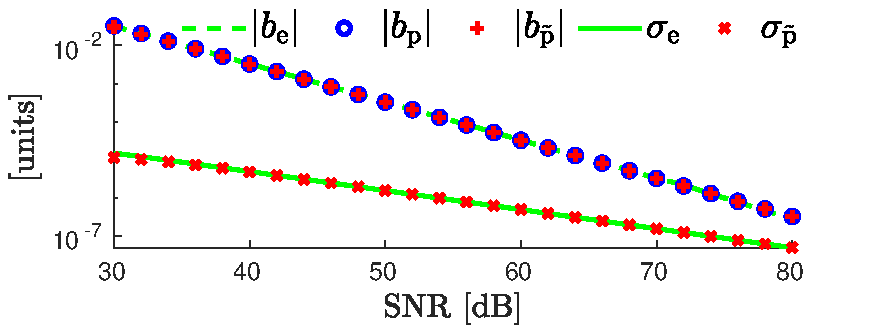
\includegraphics[width=1\textwidth]{./ChapterStatisticalAnalysis/fig/Fig_1l.pdf} 
 %   \end{minipage}
 %   \begin{minipage}{0.45\textwidth}
  %      \centering
        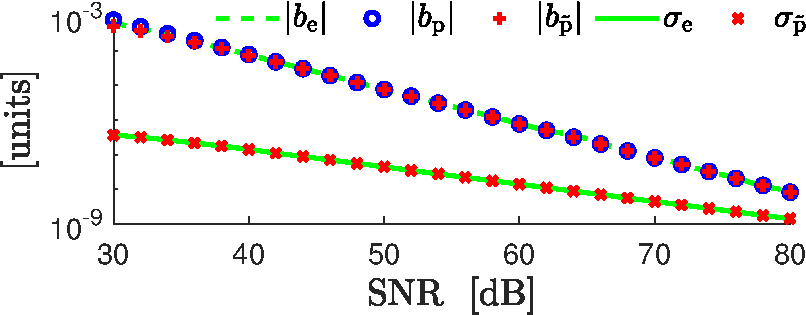
\includegraphics[width=1\textwidth]{./ChapterStatisticalAnalysis/fig/Fig_1r.pdf} 
   % \end{minipage}
  \caption{ \label{bias_sigma_NMC_unstr_str_n2} We observe the results of the LS solutions for the unstructured (left) and the structured (right) EIV problems. These results are the empirical bias $b_{\mathrm{e}}$, the predicted bias from exact data $b_{\mathrm{p}}$, the predicted bias from observed data $b_{\widetilde{\mathrm{p}}}$, the empirical standard error $\sigma_{\mathrm{e}}$, and the standard error from the estimations using observed data $\sigma_{\widetilde{\mathrm{p}}}$. The estimation biases are proportional to the perturbation variance and the estimation standard errors are proportional to the perturbation standard deviation. Since the standard errors are smaller than the biases, the MC simulation is meaningful. }
\end{figure}

The absolute and relative errors between the predicted and the empirical bias are shown in Figure \ref{fig:b_bt_abse_rele_unstr_e7}. 
The absolute errors decrease with respect to the perturbation variance.
The relative errors are lower than 5\% for SNR between 30 dB and 70 dB. 
There is an increment in the relative errors for SNR above 55 dB. 
 As the SNR increases, the empirical and the predicted bias decrease, as well as the bias error between them.
In order to reveal the bias error, more Monte Carlo runs are needed to reduce the uncertainty of the Monte Carlo simulation that depends on the square root of $N_{\mathrm{MC}}$, see Equation (\ref{eqn:stderr}).
If $N_{\mathrm{MC}}$ is insufficient, the uncertainty of the Monte Carlo simulation hides the bias error and we see this increasing effect of the relative errors. 

\begin{figure}[htb!]
    \centering
    \begin{minipage}{0.45\textwidth}
        \centering
        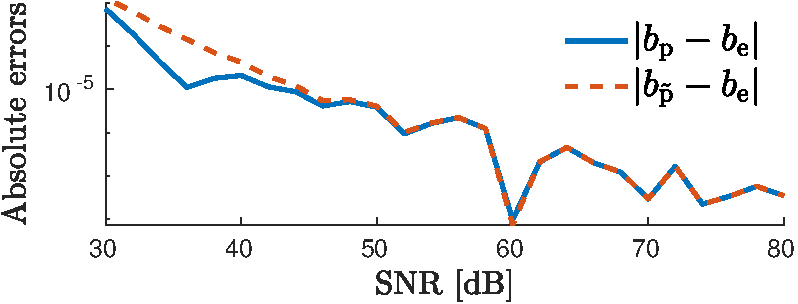
\includegraphics[width=1\textwidth]{./ChapterStatisticalAnalysis/fig/Fig_2l.pdf} 
    \end{minipage}
    \begin{minipage}{0.45\textwidth}
        \centering
        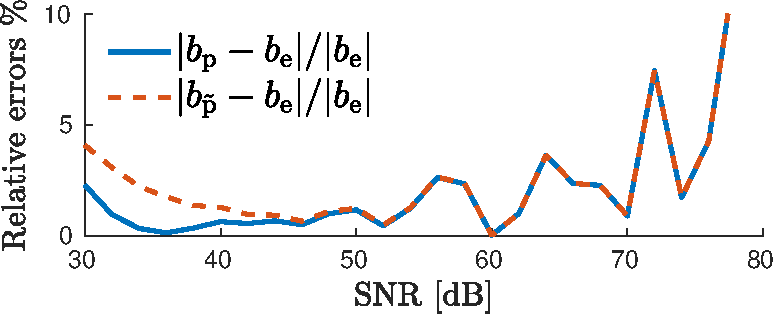
\includegraphics[width=1\textwidth]{./ChapterStatisticalAnalysis/fig/Fig_2r.pdf} 
    \end{minipage}
  \caption{ \label{fig:b_bt_abse_rele_unstr_e7} The MC simulation shows that when we solve an unstructured EIV problem with LS, the absolute errors (left) between the predicted bias and the empirical bias are proportional to the perturbation noise variance as it is expected, and the relative errors (right) are smaller than 5\% for SNR below 70 dB. The bias prediction computed from exact data ${b}_\mathrm{p}$ is very similar to that computed using observed data $b_{\widetilde{\mathrm{p}}}$. } 
\end{figure}

The errors between the predicted and the empirical variance are shown in Figure \ref{fig:v_vt_abse_rele_unstr_e7}.
The absolute and relative errors decrease with respect to the perturbation variance.
The relative errors are lower than 5\% for SNR above 40 dB. 

\begin{figure}[htb!]
    \centering
    \begin{minipage}{0.45\textwidth}
        \centering
        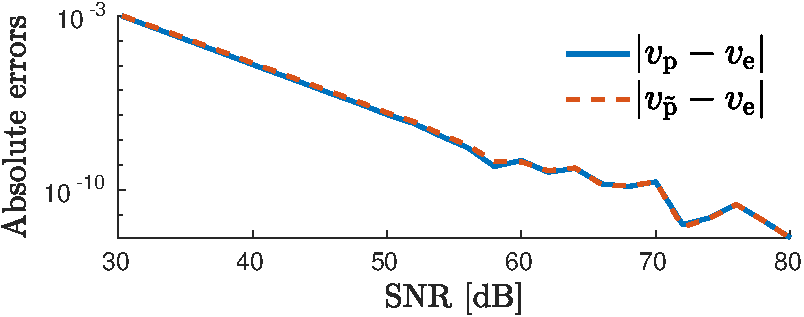
\includegraphics[width=1\textwidth]{./ChapterStatisticalAnalysis/fig/Fig_3l.pdf} 
    \end{minipage}
    \begin{minipage}{0.45\textwidth}
        \centering
        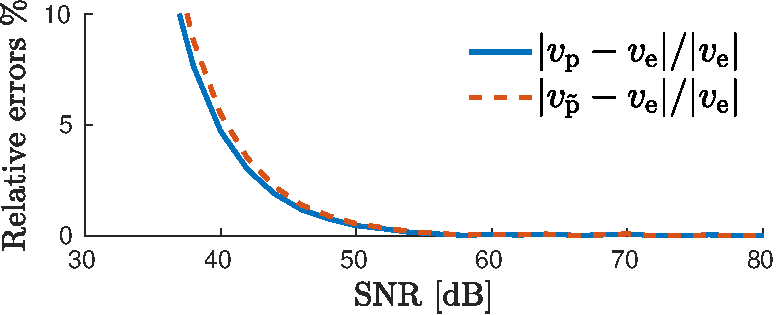
\includegraphics[width=1\textwidth]{./ChapterStatisticalAnalysis/fig/Fig_3r.pdf} 
    \end{minipage}
  \caption{ \label{fig:v_vt_abse_rele_unstr_e7} The MC simulation shows that when we solve an unstructured EIV problem with LS, the absolute errors (left) between the predicted variances and the empirical variance are proportional to the perturbation noise variance, and the relative errors (right) are smaller than 5\% for SNR higher that 40 dB. The variance prediction computed using exact data ${v}_\mathrm{p}$ is very similar to that computed from observed data $v_{\widetilde{\mathrm{p}}}$. } 
\end{figure}

Figure \ref{fig:bv_btvt_abse_rele_unstr_e7} shows the absolute and the relative errors between the predictions computed from observed data and those computed from exact data.
The absolute errors between both predictions are proportional to the perturbation noise variance.
The bias and variance predictions, from either exact data or observed data, are equivalent for SNR above 35 dB since the relative errors are lower than 5\%.
The substitution of observed data on the prediction formulas is a valid procedure that allows the prediction of the estimate statistics.

\begin{figure}[htb!]
    \centering
    \begin{minipage}{0.45\textwidth}
        \centering
        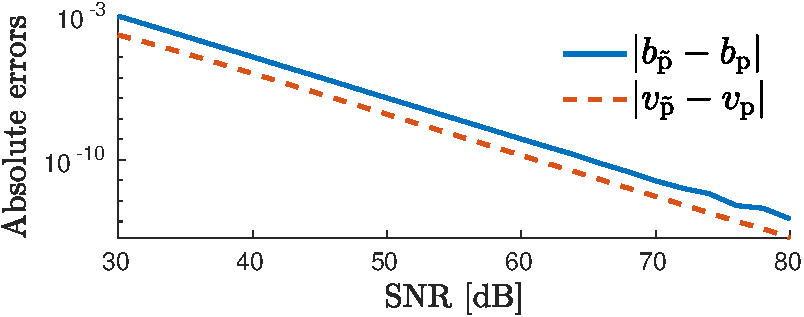
\includegraphics[width=1\textwidth]{./ChapterStatisticalAnalysis/fig/Fig_4l.pdf} 
    \end{minipage}
    \begin{minipage}{0.45\textwidth}
        \centering
        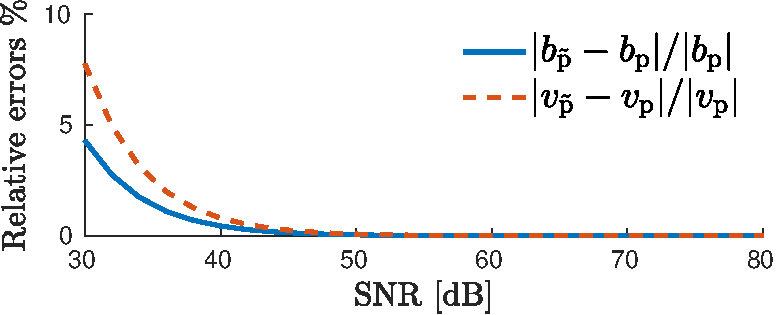
\includegraphics[width=1\textwidth]{./ChapterStatisticalAnalysis/fig/Fig_4r.pdf} 
    \end{minipage}
  \caption{ \label{fig:bv_btvt_abse_rele_unstr_e7} The MC simulation shows that when we solve an unstructured EIV problem with LS, the absolute errors (left) between the prediction with observed data and the prediction with exact data are proportional to the perturbation noise variance. The use of observed data instead of exact data in the prediction formulas is valid when the SNR is above 35 dB since the relative errors (right) are smaller than 5\%. } 
\end{figure}


\subsection{Monte Carlo simulation results for a structured EIV problem with correlated perturbations}

The MC simulation of the structured EIV problem (\ref{eqn:min_ls}) solution was conducted processing $T = 200$ samples of the transient response $\widetilde{\mathbf{y}}$ generated by a linear time invariant system of order $n = 2$, after a step input excitation with $u = 1 \ \mathrm{units}$, where the units represent any physical quantity. 
The processed step response is shown in Figure \ref{fig:y}.
The steady state response of the system is reached after 400 samples because from there on the relative error between the instantaneous values of the transient response and the steady-state response value is smaller than 2\%.
Processing 200 samples ensures that the step input estimation is computed from transient data only.
%In the following results we focus our interest in the first element of the estimate $\widehat{\mathbf{x}}_{\left[1\right]}$, where the step input level estimate $\widehat{u}$ is located.

\begin{figure}[htb!]
\centering
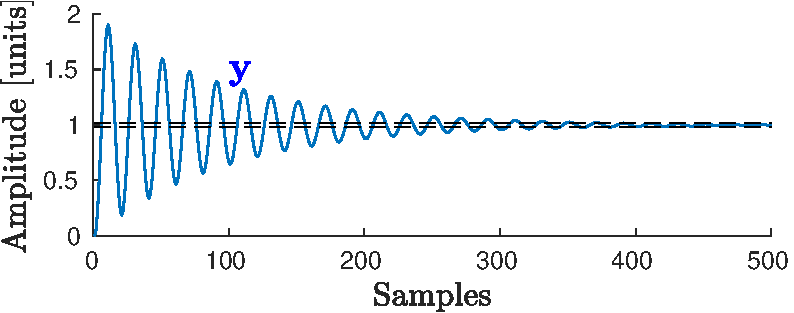
\includegraphics[width=0.5\textwidth]{./ChapterStatisticalAnalysis/fig/Fig_5.pdf} 
\caption{ \label{fig:y} The structured EIV problem is constructed with 200 samples of the step response to ensure that only transient data is used. The relative errors between the values of $\mathbf{y}$ and the steady state value are smaller than 2\% after 400 samples, as it is indicated with dashed lines. } 
\end{figure}

The empirical bias is the sample mean of the $N_{\mathrm{MC}}$ estimates minus the true value
 \begin{equation} {b}_\mathrm{e} = \frac{1}{N_{\mathrm{MC}}} \sum_{i=1}^{N_{\mathrm{MC}}}{ \widehat{u}_i - u } \approx \mu \left( \widehat{u} \right) - u. \end{equation}
The standard error associated to this empirical bias estimation \cite{Hammersley75} is defined as 
\begin{equation} \sigma_\mathrm{e} = \frac{\sigma \left( \widehat{u} \right) }{\sqrt{N_{\mathrm{MC}}}}, \quad \mathrm{where} \quad \sigma^2 \left( \widehat{u} \right) = \frac{1}{N_{\mathrm{MC}}-1} \sum_{i=1}^{N_{\mathrm{MC}}}{ \left( { \widehat{u}}_i - \mu \left( \widehat{u} \right) \right)^2 } . \end{equation} 

The plots on the right side of Figure \ref{bias_sigma_NMC_unstr_str_n2} show the empirical bias, the bias predictions (\ref{eqn:biasE}) and (\ref{eqn:biasST}), and their corresponding standard errors, for the structured EIV problem.
The empirical bias $b_\mathrm{e}$ is proportional to the perturbation noise variance, and
the bias predictions $b_\mathrm{p}$ and $b_{\widetilde{\mathrm{p}}}$ coincide with the empirical bias $b_\mathrm{e}$ only for SNR above 40 dB.
This indicates that the SNR drops to a point where the constraint $\| \mathbf{M} \| < 1$ is no longer satisfied.
At an SNR of 30 dB the perturbation noise affects the bias prediction from observed data and it is three times smaller than the empirical bias.


The absolute and relative errors between the predicted and the empirical bias are shown in Figure \ref{fig:b_bt_abse_rele_str_e7}.
It can be seen that the absolute errors are proportional to the perturbation variance, and the relative errors are lower than 5\% for SNR higher than 40 dB. 
%Nevertheless, the perturbation SNR in practical applications is not high and is near 40 dB

\begin{figure}[htb!]
    \centering
    \begin{minipage}{0.45\textwidth}
        \centering
        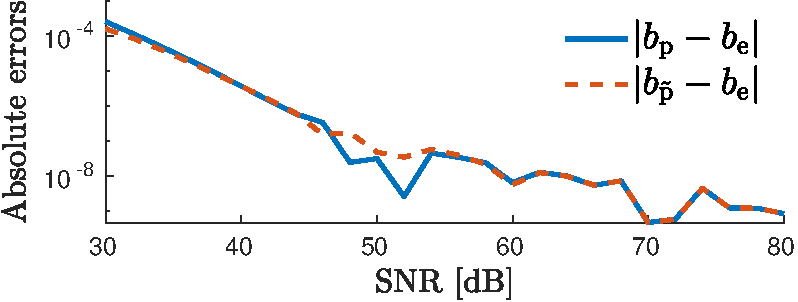
\includegraphics[width=1\textwidth]{./ChapterStatisticalAnalysis/fig/Fig_6l.pdf} 
    \end{minipage}
    \begin{minipage}{0.45\textwidth}
        \centering
        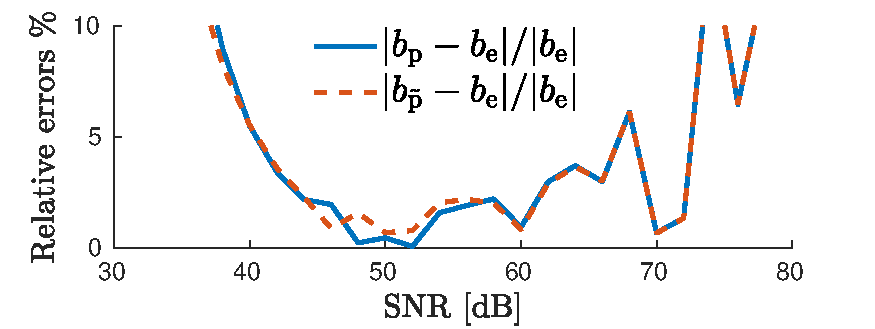
\includegraphics[width=1\textwidth]{./ChapterStatisticalAnalysis/fig/Fig_6r.pdf} 
    \end{minipage}
  \caption{ \label{fig:b_bt_abse_rele_str_e7} The MC simulation shows that when we solve a structured EIV problem with LS, the absolute errors (left) between the predicted bias and the empirical bias $b_{\mathrm{e}}$ are proportional to the perturbation noise variance, and the relative errors (right) are smaller than 5\% only for SNR above 40 dB.}
\end{figure}


The absolute and relative errors between the empirical and the predicted variance, equations (\ref{eqn:varE}) and (\ref{eqn:varST}), are shown in Figure \ref{fig:v_vt_abse_rele_str_e7}.
These absolute errors are proportional to the perturbation noise variance, whereas
the relative errors are lower than 5\% for SNR higher than 45 dB. 

The absolute and relative errors between the two predictions from observed data and from exact data, are shown in Figure \ref{fig:bv_btvt_abse_rele_str_e7}.
These absolute errors are also proportional to the perturbation noise variance, and
the relative errors show that the bias and variance predictions from either of the two alternatives are equivalent for SNR higher than 45 dB.

\begin{figure}[htb!]
    \centering
    \begin{minipage}{0.45\textwidth}
        \centering
        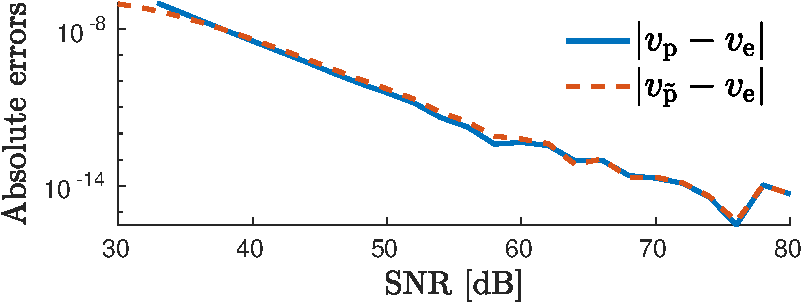
\includegraphics[width=1\textwidth]{./ChapterStatisticalAnalysis/fig/Fig_7l.pdf} 
    \end{minipage}
    \begin{minipage}{0.45\textwidth}
        \centering
        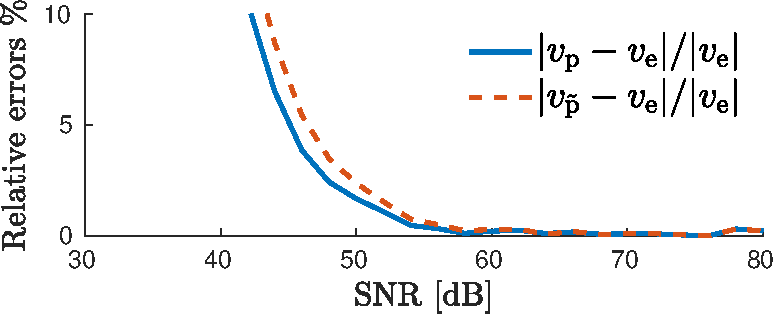
\includegraphics[width=1\textwidth]{./ChapterStatisticalAnalysis/fig/Fig_7r.pdf} 
    \end{minipage}
  \caption{ \label{fig:v_vt_abse_rele_str_e7} The MC simulation shows that when we solve a structured EIV problem with LS, the absolute errors (left) between the predicted and the empirical variance are proportional to the perturbation variance, and the relative errors (right) between the predicted and the empirical variance are smaller than 5\% for SNR above 45 dB. }
\end{figure}

\begin{figure}[htb!]
    \centering
    \begin{minipage}{0.45\textwidth}
        \centering
        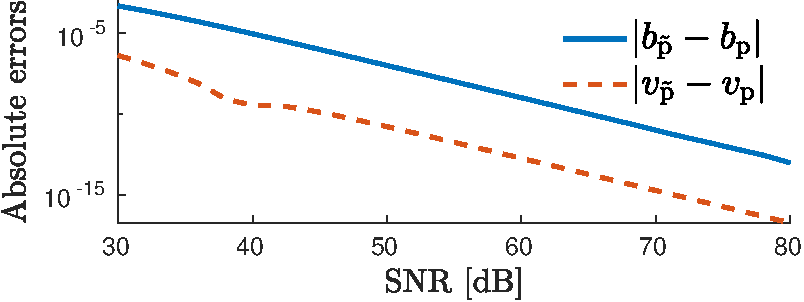
\includegraphics[width=1\textwidth]{./ChapterStatisticalAnalysis/fig/Fig_8l.pdf} 
    \end{minipage}
    \begin{minipage}{0.45\textwidth}
        \centering
        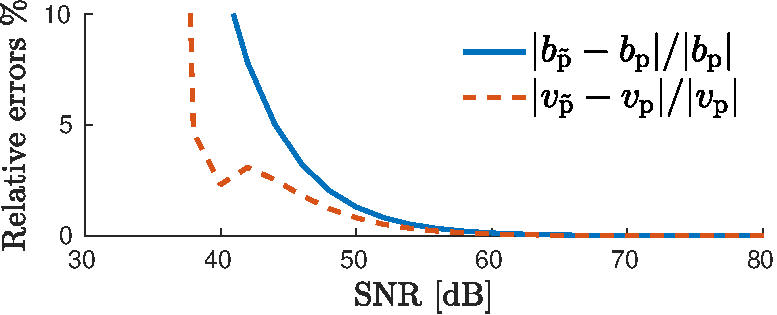
\includegraphics[width=1\textwidth]{./ChapterStatisticalAnalysis/fig/Fig_8r.pdf} 
    \end{minipage}
  \caption{ \label{fig:bv_btvt_abse_rele_str_e7} The MC simulation shows that when we solve a structured EIV problem with LS, the absolute errors (left) between the predictions computed from observed data and those from exact data are proportional to the perturbation noise variance. According to the relative errors (right), the substitution is valid for SNR higher than 45 dB. } 
\end{figure}

The simulation results show that the LS solution of the structured and correlated EIV problem is more sensitive to the perturbation.
This represents a low limit in the SNR interval imposed by the noise level.
In practical applications it is common to have SNRs of 40 dB and the user needs to be aware of the prediction error that the method has.
We measure this prediction error with the mean squared error (MSE), defined as
\begin{equation} \mathrm{MSE} = \sigma^2 + b^2. \end{equation}
 By comparing the different MSEs to the CRLB of the structured EIV problem,
Figure \ref{fig:MSE_CRLB} shows that the MSEs has the same proportionality as the CRLB with respect to the disturbing noise variance.
The MSEs are three times larger than the CRLB.
Since the difference between $\mathrm{MSE}_{\widetilde{\mathrm{p}}}$ and the CRLB is lower than one order of magnitude, 
the LS estimation of the structured EIV problem produces results that are comparable to the ML estimation.
The $\mathrm{MSE}_{\widetilde{\mathrm{p}}}$ computed from observed data approaches the CRLB for SNR below 40 dB.
This is due to the constraint violation of the Taylor series expansion.


\begin{figure}[!htpb]
\centering
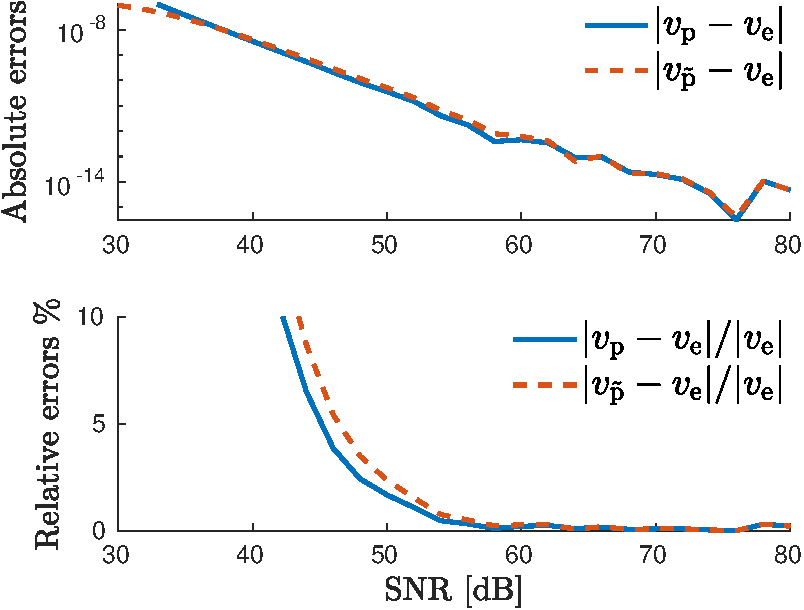
\includegraphics[width=0.5\textwidth]{./ChapterStatisticalAnalysis/fig/Fig_9.pdf}
\caption{\label{fig:MSE_CRLB}
The mean squared errors of the LS estimate are close to the Cram\'er-Rao lower bound. This is a positive indication of the goodness of the LS estimator for the structured EIV problem. The mean squared error of the empirical estimates is represented by $\mathrm{MSE}_{\mathrm{e}}$, and those of the predictions are $\mathrm{MSE}_{\mathrm{p}}$ and $\mathrm{MSE}_{\widetilde{\mathrm{p}}}$. The $\mathrm{MSE}_{\widetilde{\mathrm{p}}}$ is smaller than CRLB below 40 dB of SNR because of the introduced bias error, but the difference between $\mathrm{MSE}_{\widetilde{\mathrm{p}}}$ and the CRLB is lower than one order of magnitude.}
\end{figure}


\section{Conclusions}

 We conducted a statistical analysis of a structured errors-in-variables (EIV) estimation problem with correlation to find the first and second moments of its least-squares solution.
This estimation problem occurs in metrology when we estimate the value of a measurand directly from the sensor transient response.
The data-driven estimation of the physical quantity is formulated as a structured EIV problem with correlation that uses the observed transient response to construct both the regression matrix and the regressor.
The real-time implementation of the method uses a recursive least squares algorithm that is simple and has low computational complexity.
The assessment of the uncertainty is done using the estimate bias and variance.

The conducted statistical analysis produced expressions that predict the estimate bias and variance for given sample size and perturbation level of the observed response.
The Monte Carlo simulation validated the predictions.
We compared the results of solving an unstructured and uncorrelated EIV problem with a structured and correlated EIV problem to understand how the structure and the correlation impacts in the estimation.
We found that the predictions in the structured case are more susceptible to perturbations.
This is due to the two approximations involved, a second-order Taylor series expansion of the estimate, and the substitution of perturbed data on the prediction expressions.
The relative error results indicate that the estimate bias, and variance are predicted using the derived expressions, and the observed data.
The mean squared error of the estimate is close to the results of the maximum likelihood estimate given by the Cram\'er-Rao lower bound.

The bias and variance can be accurately predicted, provided that the Taylor series expansion is valid.
This constraint has to be taken into account to ensure the effectiveness of the method in practical applications.
In the example, it was observed that when the SNR lies outside the validity region, the bias and variance estimation was at most three times larger than the empirical values.

The methodology presented in this paper can be applied to estimate the uncertainty of the solutions to other structured EIV problems.
The bias and variance expressions obtained after the statistical analysis depend on each specific structure.




\section{STATISTICAL ANALYSIS - Ramp input}


\subsubsection{Statistical analysis of the subspace method}

To obtain the first and second moments of the step input estimate $\widehat{u}$, we need to study the solution
\begin{equation} \widehat{\mathbf{x}} = ( \mathbf{K}^\top \mathbf{W} \mathbf{K}  )^{-1} \mathbf{K}^\top \mathbf{W} \mathbf{y} , \label{eqn:xhat} \end{equation}
of the overdetermined structured errors-in-variables EIV problem (\ref{eqn:min_ewrls}).
Using a second order Taylor series expansion of the inverse matrix we can approximate the LS solution as
\begin{equation} \widehat{\mathbf{x}} \approx \left( \mathbf{I} - \mathbf{M} + \mathbf{M}^2 \right) \mathbf{C}^{-1} (\widebar{\mathbf{K}} + \mathbf{E})^\top \mathbf{W} (\widebar{\mathbf{y}} + \bm{\epsilon}). \label{eqn:xhatexp} \end{equation} 
where 
\begin{equation} \widebar{\mathbf{C}} = \widebar{\mathbf{K}}^\top \mathbf{W} \widebar{\mathbf{K}}, \quad \text{and} \quad \mathbf{M} = \widebar{\mathbf{C}}^{-1} ( \widebar{\mathbf{K}}^\top \mathbf{W} \mathbf{E} + \mathbf{E}^\top \mathbf{W} \widebar{\mathbf{K}} + \mathbf{E}^\top \mathbf{W} \mathbf{E} ). \end{equation} 

The Taylor series approximation of $\widehat{\mathbf{x}}$ enables the calculation of the estimate bias and covariance since the measurement noise $\bm{\epsilon}$ and $\mathbf{E}$ are no more subject to matrix inversion. 
The bias and the covariance of the estimate $\widehat{\mathbf{x}}$ are obtained from
\begin{equation}  \mathbf{b} \left(\widehat{\mathbf{x}} \right) = \mathbf{\mu} - \widebar{\mathbf{x}}, \label{eqn:biasdef} \end{equation}
\begin{equation} \begin{aligned} \mathrm{\mathbf{Cov}} \left( \widehat{\mathbf{x}} \right) & = \mathbb{E} \left\{ \left( \widehat{\mathbf{x}} - \mathbf{\mu} \right)  \left( \widehat{\mathbf{x}} - \mathbf{\mu} \right)^\top \right\} . \end{aligned} \label{eqn:covdef} \end{equation} 
where $\mathbf{\mu} = \mathbb{E} \left\{ \widehat{\mathbf{x}} \right\}$ is the expected value of the estimate and $\widebar{\mathbf{x}}$ is the true value. 
Considering the structure of the EIV problem, the bias and the covariance of the estimate approximation (\ref{eqn:xhatexp}) can be expressed as
\begin{equation} \begin{aligned} \widebar{\mathbf{b}}_{\mathrm{p}} \left( \widehat{x} \right) & \approx \widebar{\mathbf{C}}^{-1} \left(  \left( \widebar{\mathbf{K}}^\top \mathbf{W} \widebar{\mathbf{B}}_1 - \widebar{\mathbf{B}}_2 \right) \mathbf{x} - \left( \widebar{\mathbf{K}}^\top \mathbf{W} \widebar{\mathbf{B}}_3 - \widebar{\mathbf{B}}_4 \right) \right), \end{aligned} \label{eqn:biasE} \end{equation}
\begin{equation} \begin{aligned} \widebar{\mathrm{\mathbf{Cov}}}_{\mathrm{p}} \left( \widehat{\mathbf{x}} \right) & \approx \widebar{\mathbf{K}}^\dagger \mathbf{W} \left( \sigma_{\epsilon}^2 \mathbf{I}_{T-n} + \widebar{\mathbf{C}}_1 - \widebar{\mathbf{C}}_2 - \widebar{\mathbf{C}}_2^\top \right) \mathbf{W} \widebar{\mathbf{K}}^{\dagger \top}  - \widebar{\mathbf{b}}_{\mathrm{p}} \left( \widehat{x} \right) \widebar{\mathbf{b}}_{\mathrm{p}}^\top \left( \widehat{x} \right), \end{aligned} \label{eqn:varE} \end{equation}
where $\widebar{\mathbf{B}}_1 = \mathbb{E} \Big\{ \mathbf{E} \widebar{\mathbf{K}}^\dagger \mathbf{W} \mathbf{E} \Big\}$, $\widebar{\mathbf{B}}_2 = \mathbb{E} \Big\{ \mathbf{E}^\top \mathbf{W} \widebar{\mathbf{P}}_\perp \mathbf{E} \Big\}$, $\widebar{\mathbf{B}}_3 = \mathbb{E} \Big\{ \mathbf{E} \widebar{\mathbf{K}}^\dagger \mathbf{W} \bm{\epsilon} \Big\}$, $\widebar{\mathbf{B}}_4 = \mathbb{E} \Big\{ \mathbf{E}^\top \mathbf{W} \widebar{\mathbf{P}}_\perp \bm{\epsilon} \Big\}$, $\widebar{\mathbf{C}}_1 = \mathbb{E} \Big\{ \mathbf{E} \mathbf{x} \mathbf{x}^\top \mathbf{E}^\top \Big\}$, \linebreak $\widebar{\mathbf{C}}_2 = \mathbb{E} \Big\{ \mathbf{E} \mathbf{x} \bm{\epsilon}^\top \Big\}$, $\widebar{\mathbf{P}}_\perp = \mathbf{I} - \widebar{\mathbf{K}} \widebar{\mathbf{K}}^\dagger \mathbf{W}$, and $\mathbf{K}^\dagger$ is the pseudo-inverse matrix of $\mathbf{K}$. 

The bias and covariance given by expressions (\ref{eqn:biasE}) and (\ref{eqn:varE}) depend on the unobservable true values $\widebar{\mathbf{x}}$ and $\widebar{\mathbf{K}}$.
The measured observations are in the sensor step response $\mathbf{y}$, and from its observations we construct $\mathbf{K}$ and compute $\widehat{\mathbf{x}}$.
The substitution of the measured data in the expressions gives an approximation of the estimate bias and covariance. 
We have then
\begin{equation} \begin{aligned} \mathbf{b}_{\mathrm{p}} \left( \widehat{\mathbf{x}} \right) & \approx \mathbf{C}^{-1} \left(  \left( \mathbf{K}^\top \mathbf{W} \mathbf{B}_1 - \mathbf{B}_2 \right) \widehat{\mathbf{x}} - \left( \mathbf{K}^\top \mathbf{W} \mathbf{B}_3 - \mathbf{B}_4 \right) \right), \end{aligned} \label{eqn:biasST} \end{equation}
  \begin{equation} \begin{aligned} {\mathrm{\mathbf{Cov}}}_{\mathrm{p}} \left( \widehat{\mathbf{x}} \right) & \approx \mathbf{K}^\dagger \mathbf{W} \left( \sigma_{\epsilon}^2 \mathbf{I}_{T-n} + \mathbf{C}_1 - \mathbf{C}_2 - \mathbf{C}_2^\top \right) \mathbf{W} \mathbf{K}^{\dagger \top} - \mathbf{b}_{\mathrm{p}} \left( \widehat{x} \right) \mathbf{b}_{\mathrm{p}}^\top \left( \widehat{x} \right), \end{aligned} \label{eqn:varST} \end{equation}
  where $\mathbf{B}_1 = \mathbb{E} \Big\{ \mathbf{E} \mathbf{K}^\dagger \mathbf{W} \mathbf{E} \Big\}$, $\mathbf{B}_2 = \mathbb{E} \Big\{ \mathbf{E}^\top \mathbf{W} \mathbf{P}_\perp \mathbf{E} \Big\}$, $\mathbf{B}_3 = \mathbb{E} \Big\{ \mathbf{E} \mathbf{K}^\dagger \mathbf{W} \bm{\epsilon} \Big\}$, $\mathbf{B}_4 = \mathbb{E} \Big\{ \mathbf{E}^\top \mathbf{W} \mathbf{P}_\perp \bm{\epsilon} \Big\}$, $\mathbf{C}_1 = \mathbb{E} \Big\{ \mathbf{E} \widehat{\mathbf{x}} \widehat{\mathbf{x}}^\top \mathbf{E}^\top \Big\}$, $\mathbf{C}_2 = \mathbb{E} \Big\{ \mathbf{E} \widehat{\mathbf{x}} \bm{\epsilon}^\top \Big\}$, and $\mathbf{P}_\perp = \mathbf{I} - \mathbf{K} \mathbf{K}^\dagger \mathbf{W}$. 

  The results of the expected values $\mathbf{B}_1$, $\mathbf{B}_2$, $\mathbf{B}_3$, $\mathbf{B}_4$, $\mathbf{C}_1$, and $\mathbf{C}_2$, were described by the authors of this paper in \cite{Quintana19}.
The bias and covariance were obtained to extend previous analysis conducted on EIV estimation problems without an imposed structure \cite{Vaccaro94, Stewart90SPT}.
It was shown that the bias and variance expressions (\ref{eqn:biasST}) and (\ref{eqn:varST}) are valid predictions of the first and second moments of the LS estimate of a Hankel structured EIV problem.
The problem formulated by the step input estimation method belongs to this type of structured EIV problems and can use the derived expressions to find the bias and variance of the input estimate $\widehat{u}$.
The bias of the estimate $\widehat{u}$ is the fist element of $\mathbf{b}_{\mathrm{p}} \left( \widehat{\mathbf{x}} \right)$ and the variance of $\widehat{u}$ is the first element in the main diagonal of $\mathrm{\mathbf{Cov}}_{\mathrm{p}} \left( \widehat{\mathbf{x}} \right)$.


\subsubsection{Cram\'er-Rao lower bound of the structured EIV problem}

To find the Cram\'er-Rao lower bound (CRLB) of the structured EIV estimation problem (\ref{eqn:min_ls}), we consider that this structured and correlated estimation problem can be expressed as a linear in the measurements problem \cite{Pintelon12Book}
\begin{equation} e (\widehat{\mathbf{x}}, \mathbf{z}) = \mathbf{M}_1( \widehat{\mathbf{x}} ) \ \mathbf{z} = \underbrace{\begin{bmatrix} \mathbf{I}_{T-n} & - \widehat{\mathbf{x}}^T \otimes \mathbf{I}_{T-n} \end{bmatrix}}_{\mathbf{M}_1( \widehat{\mathbf{x}} )} \underbrace{\begin{bmatrix} \mathbf{y} \\ \mathrm{vec} ( \mathbf{K} ) \end{bmatrix}}_{\mathbf{z}} = 0 . \label{eqn:M1vecyK} \end{equation}
where $\mathbf{z} = \widebar{\mathbf{z}} + \bm{\epsilon}_{\mathbf{z}}$.
To have the CRLB, it is necessary the existence of the true model $\mathbf{M}_1( \mathbf{x} ) \ \mathbf{z} = 0$.
The measurement perturbation $\bm{\epsilon}_{\mathbf{z}}$ is assumed to be normally distributed with covariance matrix $\mathbf{C}_{\mathbf{z}}$, and then, the loglikelihood function of the structured and correlated EIV problem is
\begin{equation} \ln{ l(\mathbf{z}, \widehat{\mathbf{z}}, \widehat{\mathbf{x}}) } = - \frac{1}{2} \left( \mathbf{z} - \widehat{\mathbf{z}} \right)^\top \mathbf{C}_{\mathbf{z}}^{-1} \left( \mathbf{z} - \widehat{\mathbf{z}} \right) + \mathrm{constant}, \end{equation}
where the elements of $\widehat{\mathbf{z}}$ are the estimated parameters of the measurements $\mathbf{z}$,  that satisfy $\mathbf{M}_1(\widehat{\mathbf{x}}) \ \widehat{\mathbf{z}} = 0$.
The size of the Fisher information matrix $\mathbf{Fi}(\mathbf{x}, \mathbf{z})$ depends on the number of unknowns in $\widehat{\mathbf{z}}$ and grows with the sample size.
However, the Fisher information matrix $\mathbf{Fi}(\mathbf{x})$ is obtained from $\mathbf{Fi}(\mathbf{x}, \mathbf{z})$, by doing inversion by parts \cite{Pintelon12Book} \S 19, and can be expressed as  
\begin{equation} \mathbf{Fi}(\mathbf{x}) = \left( \frac{\partial e (\widehat{\mathbf{x}}, \mathbf{z}) }{\partial \mathbf{x} } \right)^\top \left( \mathbf{M}_1( \mathbf{x} ) \mathbf{C}_{\mathbf{z}}  \mathbf{M}_1^\top( \mathbf{x} ) \right)^{-1}  \left( \frac{\partial e (\widehat{\mathbf{x}}, \mathbf{z}) }{\partial \mathbf{x} } \right) .
 \label{eqn:FIM}   \end{equation} 
The partial derivatives are evaluated at the true values $\mathbf{x}$. 
Thus, the covariance matrix of the measurements is

\begin{equation} \mathbf{C}_{\mathbf{z}} = \sigma_{\epsilon}^2 \begin{bmatrix} \mathbf{I}_{T-n} & \mathbf{0}_{T-n} & \mathbf{D}_1 \\ \mathbf{0}_{T-n} & \mathbf{0}_{T-n} & \mathbf{0}_{T-n \times n \left( T-n \right)}  \\  \mathbf{D}_1^\top & \mathbf{0}_{n \left( T-n \right) \times T-n} & \mathbf{D}_2  \end{bmatrix}  \label{eqn:Cz} \end{equation} 
where
\begin{equation*} \begin{aligned} \mathbf{D}_1 &= \begin{bmatrix}\mathbf{D}_{T-n \times T-n}^{1,n} & \mathbf{D}_{T-n \times T-n}^{1,n-1} & \cdots  & \mathbf{D}_{T-n \times T-n}^{1,1}\end{bmatrix}, \\ 
 \mathbf{D}_2 &= \begin{bmatrix} \mathbf{D}_{T-n \times T-n}^{2,1} & \mathbf{D}_{T-n \times T-n}^{2,0} & \cdots & \mathbf{D}_{T-n \times T-n}^{2,2-n} \\ \mathbf{D}_{T-n \times T-n}^{2,2} & \mathbf{D}_{T-n \times T-n}^{2,1} & \cdots & \mathbf{D}_{T-n \times T-n}^{2,3-n} \\ \vdots & \vdots & & \vdots \\ \mathbf{D}_{T-n \times T-n}^{2,n} & \mathbf{D}_{T-n \times T-n}^{2,n-1} & \cdots & \mathbf{D}_{T-n \times T-n}^{2,1} \end{bmatrix} , \end{aligned}  \end{equation*} 
and the matrices
$\mathbf{D}_{r \times c}^{1,k}$ and $\mathbf{D}_{r \times c}^{2,k}$  are the first and second order finite differences matricial operators of dimensions $r \times c$  starting from the subdiagonal $k$, for example \begin{equation*} 
\mathbf{D}_{2 \times 3}^{1,1} = \begin{bmatrix} 1 & -1 & 0 \\ 0 & 1 & -1 \end{bmatrix}, \ \mathrm{and} \quad \mathbf{D}_{3 \times 3}^{2,0} = \begin{bmatrix}-1 & 0 & 0 \\ 2 & -1 & 0 \\ - 1 & 2 & -1  \end{bmatrix} . \end{equation*}
 
The Cram\'er-Rao lower bound for a biased estimator of the minimization problem (\ref{eqn:min_ls}) is 
\begin{equation} \mathrm{CRLB}_{\mathrm{b}}(\mathbf{x}) = \left( \mathbf{I}_{n+1} + \frac{\partial \mathbf{b} \left( \widehat{\mathbf{x}} \right) }{\partial \mathbf{x} } \right)^\top \mathbf{Fi}^{-1}(\mathbf{x}) \left( \mathbf{I}_{n+1} + \frac{\partial \mathbf{b} \left( \widehat{\mathbf{x}} \right) }{\partial \mathbf{x} } \right), \label{eqn:CRB_EIV} \end{equation} 
whereas for an unbiased estimator, it is $\mathrm{CRLB}_{\mathrm{ub}}(\mathbf{x}) = \mathbf{Fi}^{-1}(\mathbf{x})$.





\section{STATISTICAL ANALYSIS - Experimental validation}

To obtain the first and second moments of the step input estimate $\widehat{u}$, we need to study the least-squares (LS) solution 
\begin{equation} \widehat{\mathbf{x}} = \widetilde{\mathbf{K}}^\dagger \widetilde{\mathbf{y}} = ( \widetilde{\mathbf{K}}^\top \widetilde{\mathbf{K}}  )^{-1} \widetilde{\mathbf{K}}^\top \widetilde{\mathbf{y}} , \label{eqn:xhat} \end{equation}
of the overdetermined structured errors-in-variables EIV problem (\ref{eqn:min_ls}), 
where $\widetilde{\mathbf{K}}^\dagger$ is the pseudo-inverse matrix of $\widetilde{\mathbf{K}}$.
Using a second order Taylor series expansion of the inverse matrix we can approximate the LS solution as
\begin{equation} \widehat{\mathbf{x}} \approx \left( \mathbf{I} - \mathbf{M} + \mathbf{M}^2 \right) \mathbf{Q}^{-1} (\mathbf{K}+\mathbf{E})^\top (\mathbf{y}+\bm{\epsilon}). \label{eqn:xhatexp} \end{equation} 
where 
\begin{equation} \mathbf{Q} = \mathbf{K}^\top \mathbf{K}, \quad \text{and} \quad \mathbf{M} = \mathbf{Q}^{-1} ( \mathbf{K}^\top \mathbf{E} + \mathbf{E}^\top \mathbf{K} + \mathbf{E}^\top \mathbf{E} ). \end{equation} 

The Taylor series approximation of $\widehat{\mathbf{x}}$ enables the calculation of the bias and covariance of $\widehat{\mathbf{x}}$ since the measurement noise $\bm{\epsilon}$ and $\mathbf{E}$ are no more subject to matrix inversion. 
The bias and the covariance of the estimate $\widehat{\mathbf{x}}$ are obtained from
\begin{equation}  \mathbf{b} \left(\widehat{\mathbf{x}} \right) = \mathbf{\mu} - \mathbf{x}, \label{eqn:biasdef} \end{equation}
\begin{equation} \begin{aligned} \mathrm{\mathbf{C}} \left( \widehat{\mathbf{\mathbf{x}}} \right) & = \mathbb{E} \left\{ \left( \widehat{\mathbf{x}} - \mathbf{\mu} \right)  \left( \widehat{\mathbf{x}} - \mathbf{\mu} \right)^\top \right\} . \end{aligned} \label{eqn:covdef} \end{equation} 
where $\mathbf{\mu} = \mathbb{E} \left\{ \widehat{\mathbf{x}} \right\}$, and $\mathbf{x} = \mathbf{K}^\dagger \mathbf{y}$ is the true value. 
Considering the structure of the EIV problem, the bias and the covariance of the approximation (\ref{eqn:xhatexp}) can be expressed as
\begin{equation} \begin{aligned} \mathbf{b}_{\mathrm{p}} \left( \widehat{\mathbf{x}} \right) & \approx \mathbf{Q}^{-1} \left(  \left( \mathbf{K}^\top \mathbf{B}_1 - \mathbf{B}_2 \right) \mathbf{x} - \left( \mathbf{K}^\top \mathbf{B}_3 - \mathbf{B}_4 \right) \right), \end{aligned} \label{eqn:biasE} \end{equation}
\begin{equation} \begin{aligned} \mathrm{\mathbf{C}}_{\mathrm{p}} \left( \widehat{\mathbf{x}} \right) & \approx \mathbf{K}^\dagger \left( \sigma_{\bm{\epsilon}}^2 \mathbf{I}_{T-n} + \mathbf{C}_1 - \mathbf{C}_2 - \mathbf{C}_2^\top \right) \mathbf{K}^{\dagger \top}, \end{aligned} \label{eqn:varE} \end{equation}
where $\mathbf{B}_1 = \mathbb{E} \Big\{ \mathbf{E} \mathbf{K}^\dagger \mathbf{E} \Big\}$, $\mathbf{B}_2 = \mathbb{E} \Big\{ \mathbf{E}^\top \mathbf{P}_\perp \mathbf{E} \Big\}$, $\mathbf{B}_3 = \mathbb{E} \Big\{ \mathbf{E} \mathbf{K}^\dagger \bm{\epsilon} \Big\}$, $\mathbf{B}_4 = \mathbb{E} \Big\{ \mathbf{E}^\top \mathbf{P}_\perp \bm{\epsilon} \Big\}$, $\mathbf{C}_1 = \mathbb{E} \Big\{ \mathbf{E} \mathbf{x} \mathbf{x}^\top \mathbf{E}^\top \Big\}$, \linebreak $\mathbf{C}_2 = \mathbb{E} \Big\{ \mathbf{E} \mathbf{x} \bm{\epsilon}^\top \Big\}$, and $\mathbf{P}_\perp = \mathbf{I} - \mathbf{K} \mathbf{K}^\dagger$. 

The expected values $\mathbf{B}_1$, $\mathbf{B}_2$, $\mathbf{B}_3$, $\mathbf{B}_4$, $\mathbf{C}_1$, and $\mathbf{C}_2$, were studied in \cite{Quintana19} and their results are described in the following Lemma:

\newtheorem{thm}{Theorem}
\newtheorem{lem}[thm]{Lemma}

\normalsize % \small
%   <how to set font size here to 10 px ? />

\begin{lem}{\small}\label{lem:lemma1}
Let $\mathbf{E}$ be the matrix defined in (\ref{eqn:matrixE}),
constructed from samples of the i.i.d. normally distributed random variable $\bm{\epsilon} \sim \mathcal{N}(0, \sigma_\epsilon^2)$.
For a compatible deterministic matrix $\mathbf{H}$, or vector $\mathbf{h}$, we have
\begin{equation*} \begin{aligned} 
& \mathbb{E} \left\{ \mathbf{E} \mathbf{H} \mathbf{E} \right\} = \sigma_{\bm{\epsilon}}^2 \mathbf{A}, \
\text{where} \ a_{ij} = \mathrm{tr} \left( \mathbf{H} \begin{bmatrix} 0_{T-n} & \mathbf{D}_{T-n \times n}^{2, j-i} \end{bmatrix} \right), \\
& \ \ \text{for}  \ i = 1, \cdots, T-n, \ \text{and} \ j = 2, \cdots, n+1, \ \text{and} \ a_{i1} = 0. \\
& \mathbb{E} \left\{ \mathbf{E}^\top \mathbf{H} \mathbf{E} \right\} = \sigma_{\bm{\epsilon}}^2 \mathbf{A}, \ 
\text{where} \ a_{ij} = \mathrm{tr} \left( \mathbf{H} \ \mathbf{D}_{T-n \times T-n}^{2, j-i+1} \right)  , \\
& \ \ \text{for} \ i = 2, \cdots, n+1, \ \text{and} \ j=2, \cdots, n+1 , \ \text{and} \   a_{1j} = a_{i1} = 0,  \\ 
& \mathbb{E} \left\{ \mathbf{E} \mathbf{H} \mathbf{E}^\top \right\} = \sigma_{\bm{\epsilon}}^2 \mathbf{A}, \
\text{where} \ a_{ij} = \mathrm{tr} \left( \mathbf{H} \begin{bmatrix} 0 & 0_{n}^\top \\ 0_{n} & \mathbf{D}_{n \times n}^{2, j-i+1} \end{bmatrix} \right), \\
& \ \ \text{for} \ i = 1,\cdots,T-n, \ \text{and} \ j=1,\cdots,T-n. \\ 
& \mathbb{E} \left\{ \mathbf{E} \mathbf{H} \bm{\epsilon} \right\} = \sigma_{\bm{\epsilon}}^2 \mathbf{a} , \
\text{where} \ a_i = \mathrm{tr} \left( \mathbf{H} \begin{bmatrix} 0_{T-n} & \mathbf{D}_{T-n \times n}^{1,n+1-i} \end{bmatrix} \right) , \\
& \ \ \text{for} \ i = 1,\cdots,T-n . \\
& \mathbb{E} \left\{ \mathbf{E}^\top \mathbf{H} \bm{\epsilon} \right\} = \sigma_{\bm{\epsilon}}^2 \mathbf{a}, \
\text{where} \ a_i = \ \mathrm{tr} \left( \mathbf{H} \ \mathbf{D}_{T-n \times T-n}^{1, n+2-i} \right), \\ & \ \ \text{for} \ i = 2,\cdots,n+1  , \ \text{and} \ a_1 = 0,   \\
& \mathbb{E} \left\{ \mathbf{E} \mathbf{h} \bm{\epsilon}^\top \right\} = \sigma_{\bm{\epsilon}}^2 \mathbf{Z}, \
\text{where} \ \mathbf{Z}_{j} = -\mathbf{D}_{T-n \times n+1}^{1,-j} \begin{bmatrix} & \mathbf{R}_n \\ 0 \end{bmatrix} \mathbf{h} ,  \\ 
& \ \ \text{for} \ j = 1,\cdots,T-n ,\\
\end{aligned} \end{equation*} 
where $\mathbf{R}_n$ is a reversal matrix, and the matrices
$\mathbf{D}_{r \times c}^{1,k}$ and $\mathbf{D}_{r \times c}^{2,k}$  are the first and second order finite differences matricial operators of dimensions $r \times c$  starting from the subdiagonal $k$, for example \begin{equation*} 
\mathbf{D}_{2 \times 3}^{1,1} = \begin{bmatrix} 1 & -1 & 0 \\ 0 & 1 & -1 \end{bmatrix}, \ \text{and} \quad \mathbf{D}_{3 \times 3}^{2,0} = \begin{bmatrix}-1 & 0 & 0 \\ 2 & -1 & 0 \\ - 1 & 2 & -1  \end{bmatrix} .
\end{equation*} 
\end{lem}

\normalsize

A proof of the lemma is given in the Appendix.

The bias and covariance given by expressions (\ref{eqn:biasE}) and (\ref{eqn:varE}) depend on the unobservable true values $\mathbf{x}$, $\mathbf{K}$.
The measured variable is the sensor step response $\widetilde{\mathbf{y}}$, and from its observations we construct $\widetilde{\mathbf{K}}$ and compute $\widehat{\mathbf{x}}$.
The substitution of the measured data in the expressions gives an approximation of the bias and covariance estimation.
We have then
\begin{equation} \begin{aligned} \mathbf{b}_{\widetilde{\mathrm{p}}} \left( \widehat{\mathbf{x}} \right) & \approx \widetilde{\mathbf{Q}}^{-1} \left(  \left( \widetilde{\mathbf{K}}^\top \widetilde{\mathbf{B}}_1 - \widetilde{\mathbf{B}}_2 \right) \widehat{\mathbf{x}} - \left( \widetilde{\mathbf{K}}^\top \widetilde{\mathbf{B}}_3 - \widetilde{\mathbf{B}}_4 \right) \right), \end{aligned} \label{eqn:biasST} \end{equation}
\begin{equation} \begin{aligned} \mathrm{\mathbf{C}}_{\widetilde{\mathrm{p}}} \left( \widehat{\mathbf{x}} \right) & \approx \widetilde{\mathbf{K}}^\dagger \left( \sigma_{\epsilon}^2 \mathbf{I}_{T-n} + \widetilde{\mathbf{C}}_1 - \widetilde{\mathbf{C}}_2 - \widetilde{\mathbf{C}}_2^\top \right) \widetilde{\mathbf{K}}^{\dagger \top}, \end{aligned} \label{eqn:varST} \end{equation}
where $\widetilde{\mathbf{B}}_1 = \mathbb{E} \Big\{ \mathbf{E} \widetilde{\mathbf{K}}^\dagger \mathbf{E} \Big\}$, $\widetilde{\mathbf{B}}_2 = \mathbb{E} \Big\{ \mathbf{E}^\top \widetilde{\mathbf{P}}_\perp \mathbf{E} \Big\}$, $\widetilde{\mathbf{B}}_3 = \mathbb{E} \Big\{ \mathbf{E} \widetilde{\mathbf{K}}^\dagger \bm{\epsilon} \Big\}$, $\widetilde{\mathbf{B}}_4 = \mathbb{E} \Big\{ \mathbf{E}^\top \widetilde{\mathbf{P}}_\perp \bm{\epsilon} \Big\}$, $\widetilde{\mathbf{\mathbf{C}}}_1 = \mathbb{E} \Big\{ \mathbf{E} \widehat{\mathbf{x}} \widehat{\mathbf{x}}^\top \mathbf{E}^\top \Big\}$, $\widetilde{\mathbf{C}}_2 = \mathbb{E} \Big\{ \mathbf{E} \widehat{\mathbf{x}} \bm{\epsilon}^\top \Big\}$, and $\widetilde{\mathbf{P}}_\perp = \mathbf{I} - \widetilde{\mathbf{K}} \widetilde{\mathbf{K}}^\dagger$. 

The bias and covariance were obtained to extend previous analysis conducted on EIV estimation problems without an imposed structure \cite{Vaccaro94, Stewart90SPT}.
It was shown that the bias and variance expressions (\ref{eqn:biasST}) and (\ref{eqn:varST}) are good predictions of the first and second moments of the LS estimate of a Hankel structured EIV problem.
The problem formulated by the step input estimation method belongs to this type of structured EIV problems and the derived expressions can be used to find the bias and variance of the input estimate $\widehat{u}$.
The bias and variance predictions approximate the empirical bias and variance.

The assessment of the uncertainty of the estimate $\widehat{\mathbf{x}}$ is obtained from the covariance matrix $\mathrm{\mathbf{C}}_{\widetilde{\mathrm{p}}} \left( \widehat{\mathbf{x}} \right)$. In this way, the uncertainty of the step input estimate $\widehat{u}$ is described by the variance in the first element on the diagonal of $\mathrm{\mathbf{C}}_{\widetilde{\mathrm{p}}} \left( \widehat{\mathbf{x}} \right)$.

In the rest of this section we describe the Cram\'er-Rao lower bound (CRB) of the structured EIV estimation problem (\ref{eqn:min_ls}), that can be expressed as a linear in the measurements problem \cite{Pintelon12Book}
\begin{equation} e (\widehat{\mathbf{x}}, \widetilde{\mathbf{z}}) = \mathbf{M}_1( \widehat{\mathbf{x}} ) \ \widetilde{\mathbf{z}} = \begin{bmatrix} \mathbf{I}_{T-n} & - \widehat{\mathbf{x}}^T \otimes \mathbf{I}_{T-n} \end{bmatrix} \begin{bmatrix} \widetilde{\mathbf{y}} \\ \mathrm{vec} ( \widetilde{\mathbf{K}} ) \end{bmatrix} = 0 . \label{eqn:M1vecyK} \end{equation}
where $\widetilde{\mathbf{z}} = \mathbf{z} + \epsilon_{\mathbf{z}}$.
The CRB requires that the true model $\mathbf{M}_1( \mathbf{x} ) \ \mathbf{z} = 0$ exists.
Under the assumption of the measurement perturbation $\epsilon_{\mathbf{z}}$ being normally distributed with covariance matrix $\mathbf{C}_{\mathbf{z}}$, the loglikelihood function of the structured EIV problem is
\begin{equation} \ln{ l(\widetilde{\mathbf{z}}, \widehat{\mathbf{z}}, \widehat{\mathbf{x}}) } = - \frac{1}{2} \left( \widetilde{\mathbf{z}} - \widehat{\mathbf{z}} \right)^\top \mathbf{C}_{\mathbf{z}}^{-1} \left( \widetilde{\mathbf{z}} - \widehat{\mathbf{z}} \right) + \mathrm{constant}, \end{equation}
where $\widehat{\mathbf{z}}$ are parameters of the measurements $\widetilde{\mathbf{z}}$ that have to be estimated and satisfy $\mathbf{M}_1( \widehat{\mathbf{x}} ) \ \widehat{\mathbf{z}} = 0$.
The size of the Fisher information matrix $\mathbf{Fi}(\mathbf{x}, \mathbf{z})$ depends on the number of unknowns in $\widehat{\mathbf{z}}$ and grows with the sample size.
Moreover, in Chapter 19 of \cite{Pintelon12Book} it is shown that the Fisher information matrix $\mathbf{Fi}(\mathbf{x})$ can be obtained from $\mathbf{Fi}(\mathbf{x}, \mathbf{z})$ after doing inversion by parts, giving
\begin{equation} \mathbf{Fi}(\mathbf{x}) = \left( \frac{\partial e (\widehat{\mathbf{x}}, \mathbf{z}) }{\partial \mathbf{x} } \right)^\top \left( \mathbf{M}_1( \mathbf{x} ) \mathbf{C}_{\mathbf{z}}  \mathbf{M}_1^\top( \mathbf{x} ) \right)^{-1}  \left( \frac{\partial e (\widehat{\mathbf{x}}, \mathbf{z}) }{\partial \mathbf{x} } \right) 
 \label{eqn:FIM}   \end{equation} 
where the partial derivatives are evaluated at the true values $\mathbf{x}$, and the covariance matrix of the measurements is

\begin{equation} \mathbf{C}_{\mathbf{z}} = \sigma_{\epsilon}^2 \begin{bmatrix} \mathbf{I}_{T-n} & \mathbf{0}_{T-n} & \mathbf{D}_1 \\ \mathbf{0}_{T-n} & \mathbf{0}_{T-n} & \mathbf{0}_{T-n \times n \left( T-n \right)}  \\  \mathbf{D}_1^\top & \mathbf{0}_{n \left( T-n \right) \times T-n} & \mathbf{D}_2  \end{bmatrix}  \label{eqn:Cz} \end{equation} 
where
\begin{equation*} \begin{aligned} \mathbf{D}_1 &= \begin{bmatrix}\mathbf{D}_{T-n \times T-n}^{1,n} & \mathbf{D}_{T-n \times T-n}^{1,n-1} & \cdots  & \mathbf{D}_{T-n \times T-n}^{1,1}\end{bmatrix}, \ \mathrm{
and} \\ 
 \mathbf{D}_2 &= \begin{bmatrix} \mathbf{D}_{T-n \times T-n}^{2,1} & \mathbf{D}_{T-n \times T-n}^{2,0} & \cdots & \mathbf{D}_{T-n \times T-n}^{2,2-n} \\ \mathbf{D}_{T-n \times T-n}^{2,2} & \mathbf{D}_{T-n \times T-n}^{2,1} & \cdots & \mathbf{D}_{T-n \times T-n}^{2,3-n} \\ \vdots & \vdots & & \vdots \\ \mathbf{D}_{T-n \times T-n}^{2,n} & \mathbf{D}_{T-n \times T-n}^{2,n-1} & \cdots & \mathbf{D}_{T-n \times T-n}^{2,1} \end{bmatrix} . \end{aligned}  \end{equation*} 



The Cram\'er-Rao lower bound for an biased estimator of the minimization problem (\ref{eqn:min_ls}) is given by
\begin{equation} \mathrm{CRB}_{\mathrm{b}}(\mathbf{x}) = \left( \mathbf{I}_{n+1} + \frac{\partial \mathbf{b} \left( \widehat{\mathbf{x}} \right) }{\partial \mathbf{x} } \right)^\top \mathbf{Fi}^{-1}(\mathbf{x}) \left( \mathbf{I}_{n+1} + \frac{\partial \mathbf{b} \left( \widehat{\mathbf{x}} \right) }{\partial \mathbf{x} } \right), \label{eqn:CRB_EIV} \end{equation} 
and for an unbiased estimator it is $\mathrm{CRB}_{\mathrm{ub}}(\mathbf{x}) = \mathbf{Fi}^{-1}(\mathbf{x})$



\newpage

